% !TeX root = ../main.tex

\chapter{Boltzmann熵与统计系统宏观状态}
\label{Boltzmann熵与统计系统宏观状态}

  \section{Boltzmann熵}
  \label{Boltzmann熵}

    组分$a$的\textbf{Boltzmann熵密度}定义为
    \begin{eqnarray}
        s_a (t) = - \int f(\vh, t) \ln f(\vh, t) \rmd \vh ~. \label{sa}
    \end{eqnarray}
    分布函数为漂移Maxwellian分布时,有
    \begin{eqnarray}
        f (\vh, t) = \frac{1}{\pi ^{3/2}} \frac{n_a}{\vath^3} e^{-\left (\vh - \uha \right )^2} ~. \label{fDM}
    \end{eqnarray}
    其中,$n_a$与$\vath$分别是组分$a$的粒子数密度\EQ{naMh}及动理学温度\EQ{vath};$\uha$组分$a$的归一化动理学平均速度\EQ{uaMh}。把上述方程代入方程\EQ{sa},化简得漂移Maxwellian分布时的Boltzmann熵密度为
    \begin{eqnarray}
        s_a (t) & = & \left (\frac{K_a}{m_a \vath^2 } - n_a \uha^2 \right ) - n_a \ln \left (\frac{1}{\pi ^{3/2}} \frac{n_a}{\vath^3} \right )~. \label{safDM}
    \end{eqnarray}

    把方程\EQ{safDM}两边对时间求导,合并同类项化简可得Boltzmann熵密度随时间的变化率
    \begin{eqnarray}
    \begin{aligned}
        \ddt s_a (t) \quad = \quad & \frac{1}{2 T_a} \ddt K_a - 2n_a \uha \cdot \frac{1}{\vath} \ddt \ua + n_a \left (3 - \Kha + 2\uha^2 \right ) \Rdtvath 
        \\
        - & \left [1 - \ln \left (\pi ^{3/2} \right) + \uha^2 + \ln \left (\frac{n_a}{\vath^3} \right) \right ] \ddt n_a ~. \label{dtsafDM}
    \end{aligned}
    \end{eqnarray}
    此时,速度空间具有轴对称性;应用方程\EQ{dtvath0D2V}并化简得
    \begin{eqnarray}
    \begin{aligned}
        \ddt s_a (t) \quad = \quad & \left(1 + \frac{1}{3} \uha^2 \right) \frac{1}{T_a} \ddt K_a + n_a \left(1 - \frac{1}{3} \uha^2 \right) \uha \cdot \frac{1}{\vath} \ddt \ua
        \\ 
        - & \left [\frac{5}{2} - \ln \left (\pi ^{3/2} \right) - \frac{1}{3} \left (\frac{3}{2} - \uha^2 \right) + \ln \left (\frac{n_a}{\vath^3} \right) \right ] \ddt n_a
        ~. \label{dtsafDMKa}
    \end{aligned}
    \end{eqnarray}
  当组分$a$粒子数密度随时间变化率为零,则有
    \begin{eqnarray}
    \begin{aligned}
        \ddt s_a (t) \quad = \quad & \left(1 + \frac{1}{3} \uha^2 \right) \frac{1}{T_a} \ddt K_a + n_a \left(1 - \frac{1}{3} \uha^2 \right) \uha \cdot \frac{1}{\vath} \ddt \ua
        ~. \label{dtsafDMKadtna0}
    \end{aligned}
    \end{eqnarray}

  当组分$a$平均速度为零,即Maxwellian分布的Boltzmann熵密度为
    \begin{eqnarray}
        s_a (t) & = & \frac{K_a}{m_a \vath^2 } - n_a \ln \left (\frac{1}{\pi ^{3/2}} \frac{n_a}{\vath^3} \right )~. \label{safM}
    \end{eqnarray}
  熵密度随时间的变化率为
    \begin{eqnarray}
        \ddt s_a (t) & = & \frac{1}{T_a} \ddt K_a
        - \left [\frac{7}{4} - \ln \left (\pi ^{3/2} \right) + \ln \left (\frac{n_a}{\vath^3} \right) \right ] \ddt n_a
        ~. \label{dtsafMKa}
    \end{eqnarray}
  当组分$a$粒子数密度随时间变化率为零时,Maxwellian分布的Boltzmann熵密度随时间变化率为
    \begin{eqnarray}
        \ddt s_a (t) & = & \frac{1}{T_a} \ddt K_a
        ~. \label{dtsafMKadtna0}
    \end{eqnarray}
    
  \section{熵增原理}
  \label{熵增原理}

  \section{统计系统宏观状态}
  \label{统计系统宏观状态}
  
  从方程\EQ{Kingxi0}可知,Maxwellian分布\EQ{fho}是King分布\EQ{fhl}中特征参量$\uhaz$为零时的极限情形。从第\ref{基于VFP谱方程的动理学矩方程}节可知,模型MM\EQ{fho}、KM\EQ{fhl}、MMM\EQ{fhofhos}与KMM\EQ{fhlfhls}皆是GKMM\EQ{fhlfhlsl}在不同约束条件下的特殊情形。记模型GKMM描述的系统的宏观状态为\textbf{非平衡定态}(中国大百科全书);则Maxwellian分布(MM)对应的热力学平衡态为特殊定态,记为\textbf{基态}。
  
  \subsection{均匀空间宏观态}
  \label{均匀空间平衡态}
  
  热力学平衡态、热力学准平衡态是无亚观平均运动($\uhas \equiv 0$)的定态。热力学亚平衡态等是所有特征参量与阶数$l$无关的定态。对于空间处于均匀状态的系统,常见的定态是热力学平衡态、热力学准平衡态与热力学亚平衡态。

  \subsubsection{热力学平衡态}
  \label{热力学平衡态}
  
  由方程\EQ{dtMho}可知,热力学平衡态时,系统所有动理学矩具有空间均匀性且不随时间改变;即系统达到\textbf{细致平衡}。在质心坐标系中,分布函数可用模型MM\EQ{fho}描述。由于在自碰撞过程中,系统的任意阶动理学矩的变化率都为零,因此记热力学平衡态为\textbf{无穷阶平衡}。在运动坐标系中,处于热力学平衡态的系统的分布函数可用模型KM\EQ{fhl}描述。
  
  \subsubsection{热力学准平衡态}
  \label{热力学准平衡态}
  \textbf{热力学准平衡态}:(MMM)
  
  从方程\EQ{dtna3D1V}-\EQ{dtMhj}可知,当等离子体系统处于均匀空间准平衡态时,单一组分的动量恒为零、粒子数密度保持恒定而局域温度可能随时间改变。也就是说处于\textbf{均匀空间准平衡态}时,由于Coulomb碰撞效应等离子体各组分处于动量平衡、能量有交换(温度不相同)且$j\ge3$的归一化标量矩随时间演化的状态。
  
  若有$\calRh_{2,0}^0$可以近似为零,意味着等离子体各组分温度近似不随时间改变,约定此等离子体系统处于\textbf{热力学准平衡态}。记此时为\textbf{二阶准平衡}。

  当模型MMM中所有子分布的温度相等时,此时约化为MM模型。换而言之,热力学平衡态是热力学准平衡态的特殊情形。 
  
  \subsubsection{热力学亚平衡态}
  \label{热力学亚平衡态}
  \textbf{热力学亚平衡态}:(KMM)
  
  由方程\EQ{dtna3D1V}可知,热力学亚平衡态时,系统所有动理学矩具有空间均匀性,且质量密度与动量处于平衡态(其二阶及以上动理学矩随时间改变)。记此时为\textbf{一阶平衡}。
  
  
  若要使得系统满足热平衡,即要求
  \begin{eqnarray}
      \calRh_{2,0}^0  &=&  0  ~.  \label{R202}
  \end{eqnarray}
  可证,Maxwellian分布是满足上述要求以及边界条件的一个理论解。\textbf{猜想}:除此之外,别无他解。
  
  若组分$a$的模型KMM中所有子分布具有相同的平均速度,则组分$a$处于热力学准平衡态。此时组分$a$的分布函数可以模型MMM描述;换而言之,热力学准平衡态是热力学亚平衡态\EQ{fhlfhlnTsu}的特殊情形。
  
  \subsection{非均匀空间宏观态}
  \label{非均匀空间宏观态}

  对于空间非均匀的热力学非平衡系统,采用如下局域平衡假设。
  \textbf{局域平衡假设}:
  \begin{assumption}
        如果系统状态偏离某一定态(平衡态、准平衡态或者亚平衡态)的程度不大,则可假设系统在宏观小而微观大的局域范围内处于\textbf{局域定态}(局域平衡态、局域准平衡态或者局域亚平衡态)。
  \end{assumption}

  宏观小而微观大是指每个小的区域内的性质(如T,p等)可以认为是近乎均匀的。假设把某小区域与其周围的体系隔离开来,在刚隔离开的时刻t,此小区域仍处于非平衡态,但经过极短时间dt之后,这个小区域内的分子便达到平衡分布,即可认为此区域达到热力学平衡,故可给出此小区域的所有热力学函数,并假定这套热力学量可以用来描述此局域在时刻t的热力学状态
  
  \subsubsection{局域平衡态}
  \label{局域平衡态}
  \textbf{局域平衡态}:(KM模型)
  当自碰撞过程中组分的热力学状态参量不随时间变换,则系统处于\textbf{局域平衡态}。
  
  \subsubsection{局域准平衡态}
  \label{局域准平衡态}
  \textbf{非均匀空间准平衡态}。当空间梯度足够小时,则方程\EQ{dtna}与\EQ{dtvath}忽略空间梯度项为
  \begin{eqnarray}
      \Rdtrhoa &\approx& 0, \label{dtnasub} \\
      \Rdtvath &\approx&  \frac{1}{3} \calRh_{2,0}^0 - \frac{2}{9} \uh_a \cdot \calRh_1  \left(\left \{\colhI{_a} \right \} \right)  ~.  \label{dtvathsub}
  \end{eqnarray}
  
  
  \subsubsection{局域亚平衡态}
  \label{局域亚平衡态}
  \textbf{局域亚平衡态}
  
  特别地,当组分$a$的局域平均速度恒为零时,记其处于\textbf{一阶局域亚平衡态}。若系统中所有组分的局域平均速度皆为零时,则称等离子体处于一阶局域亚平衡态。
  
  由方程\EQ{dtnasub}可知,当系统空间梯度足够小时时,则其质量密度近似不随时间改变。由于此时其动量近似平衡,记此时为\textbf{一阶局域平衡}。
  

  由方程\EQ{dtvathsub}可知,当其右边足够小时,等离子体组分$a$温度近似不随时间改变。由于此时组分$a$温度梯度亦是小量,记此状态为\textbf{局域热平衡态}。局域热平衡态为\textbf{二阶局域平衡}。

  从局域平衡态的约定可知,局域热平衡态是局域亚平衡态的一个特殊状态。
  


\chapter{Fokker-Planck方程的直接解法}
\label{Fokker-Planck方程的直接解法}

  当物理空间梯度效应以及平均电磁场效应可忽略时,此时VFP方程$\EQ{VFPhd}$约化为均匀空间0D-3V模型;即带Rosenbluth势Fokker-Planck(FP)碰撞项方程
  \begin{eqnarray}
      \ddt f \left(\vh,t \right) &=& \ddt \navthf \ = \ \navth \colha ~.\label{VFPhd0D}
  \end{eqnarray}
  上述方程在球极坐标系中的形式为
  \begin{eqnarray}
      \ddt f \left(\rmvh,\mu,\phi,t \right) &=&  \navth \colha\left(\rmvh,\mu,\phi,t \right) ~.\label{VFPhd0D3V}
  \end{eqnarray}
  当速度空间具有轴对称性且对称轴为$z$轴时,方程\EQ{VFPhd0D}可表述为
  \begin{eqnarray}
      \ddt f \left(\rmvh,\mu,t \right) &=&  \navth \colha\left(\rmvh,\mu,t \right) ~.\label{VFPhd0D2Vaxis}
  \end{eqnarray}
  
  本文中$\colha$采用归一化的FPS碰撞算子形式,即由方程\EQ{FPShda}-\EQ{CFHGh}描述。对于空间均匀等离子体,其归一化碰撞项为
  \begin{eqnarray}
      \colha \left(\vh,t \right) &=& \sum_{b=1}^{N_s} \nbvth \Gabh \colhab \label{FPShda3}
  \end{eqnarray}
  其中,
  \begin{eqnarray}
      \Gabh \left(t \right) &=& C_{\Gamma} \times 4 \pi \left(\frac{Z_a Z_b}{4 \pi \varepsilon_r m_a} \right)^2 \lnAab ~. \label{Gabh3}  \\
      \colhab \left(\vh,t \right) &=& \CFh \Fh \fh + \CHh \ddvvbth \HFh \cdot \ddbfv \fh + \CGh \ddvvbth \ddvvbth \GFh : \ddbfvh \ddbfvh \fh ~. \label{FPShdab3}
  \end{eqnarray}
  FPS碰撞算子\EQ{FPShdab3}中三个系数分别为
  \begin{eqnarray}
      \CFh=4\pi m_M,  \quad  
      \CHh=\left(1-m_M \right) \vbth / \vath, \quad 
      \CGh=\left(\vbth / \vath \right)^2 / 2
      ~. \label{CFHGh3}          
  \end{eqnarray}
  函数$\Fh=\Fh\left(\vvbth,\mu,\phi,t \right)$是归一化背景分布函数$\Fh \left(\vhb,\mu^{'},\phi^{'},t \right)$插值到粒子$a$速度空间上的归一化形式,记
  \begin{eqnarray}
      Fmapping:\Fh \left(\rmvhb,\mu^{'},\phi^{'},t \right) \to \Fh\left(\vvbth,\mu,\phi,t \right)
      ~. \label{Fmapping}          
  \end{eqnarray}
  其中,$\vvbth=\v_a / \vbth $。
  
  归一化Rosenbluth势函数$\HFh $与$\GFh$为
  \begin{eqnarray}
    \HFh &=& \int \frac{1}{\rmvh_{ab}} \Fh \left(\vh_b,t \right) \rmd \vh _b \ = \  \frac{\vbth}{n_b }  \HF, \label{Hh} \\
    \GFh &=& \int \rmvh_{ab} \Fh \left(\vh_b,t \right) \rmd \vh _b \ = \ \frac{1}{n_b \vbth} \GF ~. \label{Gh}
  \end{eqnarray}
  上式中归一化相对速率$\rmvh_{ab}=\left|\vh-\vh_b \right|$。
  对于单一背景分布函数等离子体,归一化Rosenbluths势满足速度空间Poisson方程,
  \begin{eqnarray}
      \nabla {_{\vvbth}^2} \HFh &=& - 4 \pi \Fh\left(\vvbth,\mu,\phi,t \right),  \label{PoissonHh} \\
      \nabla {_{\vvbth}^2} \GFh &=& - 2 \HFh ~. \label{PoissonGh}
  \end{eqnarray}
  计算Rosenbluth势及其前两阶梯度是求解Fokker-Planck碰撞项方程\EQ{VFPhd0D}的核心。后续小节将采用谱分析方法计算归一化势函数$\Hh$、$\Gh$及前两阶梯度;随后给出用球谐函做分解的归一化FPS碰撞算子的具体形式。

  当发生Coulomb碰撞的两种组分属于同种粒子(具有相同的质量、电荷等微观物理属性)时,FPS碰撞算子\EQ{FPShdab3}中系数$C_{\Hh}=0$。特别地,对于自碰撞过程($a=b$),两种组分具有相同的宏观物理性质(粒子数密度、宏观速度、热速度等)。FPS自碰撞算子为
  \begin{eqnarray}
      \colhaa \left(\vh,t \right) &=& 4 \pi \fh \fh + \frac{1}{2} \ddbfvh \ddbfvh \Gfh : \ddbfvh \ddbfvh \fh ~. \label{FPShdaa}
  \end{eqnarray}
  类似于等\SEC{VFP谱方程}节,下一节将给出Rosenbluth势以及归一化FPS碰撞算子的球谐函数展开形式。
  
  \section{归一化FPS碰撞算子的球谐函数展开}
  \label{归一化FPS碰撞算子的球谐函数展开}
  
  应用定理\EQ{定理-球谐函数展开},归一化背景分布函数$\Fh \left (\rmvhb,\mu,\phi,t \right)$用球谐函数做谱展开,有
  \begin{eqnarray}
      \Fh \left(\rmvhb,\mu,\phi,t \right) &=& \sumLoq \sumLnL \Fhlm \left( \rmvhb,t \right) \YLM \left(\mu, \phi \right) ~. \label{Fhsph}
  \end{eqnarray}
  类似地,归一化Rosenbluth势函数用球谐函数展开,
  \begin{eqnarray}
      \Hh \left(\vvbth,\mu,\phi ,t \right) &=& 4 \pi \sumLoq \sumLnL \Hhlm \left( \vvbth ,t \right) \YLM \left(\mu, \phi \right) , \label{Hhsph} \\
      \Gh \left(\vvbth,\mu,\phi,t \right) &=& 4 \pi \sumLoq \sumLnL \Ghlm \left( \vvbth ,t \right) \YLM \left(\mu, \phi \right) ~. \label{Ghsph}
  \end{eqnarray}

  \subsection{Rosenbluth势函数及其梯度}
  \label{Rosenbluth势函数的及其梯度}
  
  把方程\EQ{fhsph}代入方程\EQ{Hh}与\EQ{Gh},经过化简并与上述两个方程对比可得第$(L,M)$阶Rosenbluth势的振幅分别为
  \begin{eqnarray}
      \Hhlm \left(\vvbth,t \right) &=& \frac{1}{2 L + 1} \frac{1}{\vvbth} \left (\ILFhlm + \JLpFhlm \right) , \label{HhLM} \\
      \Ghlm \left(\vvbth,t \right) &=& \frac{1}{2 L + 1} \frac{1}{\vvbth} \left (\frac{\ILIIFhlm + \JLpFhlm}{2 L + 3} - \frac{\ILFhlm + \JLnFhlm}{2 L - 1} \right)  ~. \label{GhLM}
  \end{eqnarray}
  其中,函数$\IjFhlm$与$\JjFhlm$分别是背景归一化分布函数$\Fhlm\left(\rmvhb,t \right)$的变上/下限积分,采用\textbf{Shkarofsky积分}\cite{Shkarofsky1967,Shkarofsky1997}形式,
  \begin{eqnarray}
      \IjFhlm \left(\vvbth,t \right) &=& I_j\left(\Fhlm \right) \ = \ \frac{1}{\vvbth^j} \int_0^{\vvbth} \rmvhb^{j+2} \Fhlm \left( \rmvhb,t \right) \rmd \rmvhb, \label{IjFLM} \\ 
      \JjFhlm \left(\vvbth,t \right) &=& J_j\left(\Fhlm \right) \ = \ \vvbth^j \int_{\vvbth}^{\infty} \frac{\rmvhb^2}{\rmvhb^j} \Fhlm \left( \rmvhb,t \right) \rmd \rmvhb ~. \label{JjFLM}
  \end{eqnarray}
  
  根据Shkarofsky积分的定义,其前两阶关于速度轴$\vvbth$的偏导数分别为
  \begin{eqnarray}
      \ddscrvh \IjFhlm \left(\vvbth,t \right) &=&  \vvbth^2 \Fhlm - \frac{j}{\vvbth} \IjFhlm, \quad j = L,L+2, \label{dIjFLM} \\
      \ddscrvh \JjFhlm \left(\vvbth,t \right) &=&  - \vvbth^2 \Fhlm + \frac{j}{\vvbth} \JjFhlm, \quad j = L-1,L+1 \label{dJjFLM}
  \end{eqnarray}
  以及
  \begin{eqnarray}
  \begin{aligned}
      \dddscrvh \IjFhlm \left(\vvbth,t \right) \quad = \quad & - \left(j-2 \right)  \vvbth \Fhlm + \frac{j(j+1)}{\vvbth^2} \IjFhlm 
      \\ & + \vvbth^2 \ddscrvh \Fhlm, \quad j = L,L+2, \label{ddIjFLM} \\
      \dddscrvh \JjFhlm \left(\vvbth,t \right) \quad = \quad & - \left(j+2 \right) \vvbth \Fhlm + \frac{j (j-1)}{\vvbth^2} \JjFhlm 
      \\ & - \vvbth^2 \ddscrvh \Fhlm, \quad j = L-1,L+1 . \label{ddJjFLM}
  \end{aligned}
  \end{eqnarray}
  其中,函数$\Fhlm=\Fhlm\left(\vvbth,t \right)$是归一化背景分布函数的第$(L,m)$阶振幅$\Fhlm \left(\vhb,t \right)$插值到粒子$a$速度空间上的归一化形式,记
  \begin{eqnarray}
      F_L^M mapping:\Fhlm \left(\rmvhb,t \right) \to \Fhlm \left(\vvbth,t \right)
      ~. \label{FLMmapping}          
  \end{eqnarray}
  
  对方程\EQ{HhLM}与\EQ{GhLM}两边做关于速度轴$\vvbth$的一次求导,结合方程\EQ{dIjFLM}-\EQ{ddJjFLM},经过合并同类项化简可得Rosenbluth势函数振幅关于速度轴方向的一阶偏导数分别为
  \begin{eqnarray}
      \ddscrvh \Hhlm &=& \frac{1}{2 L + 1} \frac{1}{\vvbth^2} \left [-(L+1) \ILFhlm + (L) \JLpFhlm \right] , \label{dvHhLM} \\
      \ddscrvh \Ghlm &=& \frac{(L-1) \ILFhlm - (L) \JLnFhlm}{(2 L -1) (2 L +1 )} - \frac{(L+1) \ILIIFhlm - (L+2) \JLpFhlm}{(2 L + 1) (2 L + 3 )} ~. \label{dvGhLM}
  \end{eqnarray}
  类似地,Rosenbluth势函数振幅关于速度轴方向的二阶偏导数分别为
  \begin{eqnarray}
      \dddscrvh \Hhlm &=& - \Fhlm + \frac{1}{\vvbth^3} \left [\frac{(L+1) (L+2)}{2 L + 1} \ILFhlm + \frac{L (L-1) }{2 L + 1} \JLpFhlm \right] ~. \label{ddvHhLM} \\
      \dddscrvh \Ghlm &=& {C_G^{n2}}_L \left(\ILFhlm + \JLnFhlm \right) + {C_G^{p2}}_L \left(\ILIIFhlm + \JLpFhlm \right)~. \label{ddvGhLM}
  \end{eqnarray}
  其中,系数${C_G^{n2}}_L$与${C_G^{p2}}_L$分别为
  \begin{eqnarray}
      {C_G^{n2}}_L &= & - \frac{L(L-1)}{(2L-1) (2L+1)} , \label{CG2L} \\ 
      {C_G^{p2}}_L &= & \frac{(L+1) (L+2)}{(2L+1) (2L+3)}  ~. \label{CG2L2}
  \end{eqnarray}
  
    球极坐标其三个基矢分别记为$ \left(\bfe_{\vh}, \bfe_{\mu}, \bfe_{\phi} \right) = \left(\bfe_1, \bfe_2, \bfe_3 \right)$。应用球极坐标系中梯度\EQ{gradsp}与二阶梯度算符\EQ{gradgradspup},可以得到方程\EQ{FPShdab3}中归一化Rosenbluth势函数的梯度以及$\Gh$函数的二阶梯度。

  当系统速度空间具有轴对称性并且取球极坐标系极轴($z$)与对称轴重合时,归一化Rosenbluth势函数的梯度分别为
  \begin{eqnarray}
      \frac{1}{4\pi} \ddvvbth  \Hh &=& \ex \sumLoq \PL \ddscrvh \Hhlm + \ey \sumLIq \frac{1}{\vvbth} \Hhlm \PLI , \label{ddHhAxis} 
      \\
      \frac{1}{4\pi} \ddvvbth  \Gh &=& \ex \sumLoq \PL \ddscrvh \GhL + \ey \sumLIq \frac{1}{\vvbth} \GhL \PLI ~. \label{ddGhAxis}
  \end{eqnarray}
  $\Gh$函数的二阶梯度可表述为
  \begin{eqnarray}
  \begin{aligned}
      \frac{\vvbth}{4\pi} \ddvvbth \ddvvbth  \Gh \ = \ & \ex \ex \vvbth \sumLoq \PL \dddscrvh \GhL - 
      \left(\ex \ey + \ey \ex \right) \sumLIq \left ( \frac{\GhL}{\vvbth} - \dddscrvh \GhL \right ) \PLI 
      \\
      + &  \ey \ey \sumLoq \left[\left(\PLII + \frac{\mu}{\sinQ} \PLI \right) \frac{\GhL}{\vvbth} + \PL \ddscrvh \GhL \right] 
      \\
      + & \ez \ez \sumLoq \left (\frac{\mu}{\sinQ} \PLI \frac{\GhL}{\vvbth} +  \PL \ddscrvh \GhL \right) , \label{dddGhAxis} 
  \end{aligned}
  \end{eqnarray}

  特别地当等离子体背景组分处于准热平衡态,速度空间具有球对称性,此时归一化Rosenbluth势函数的梯度分别为
  \begin{eqnarray}
      \ddvvbth  \Hh \left (\vvbth,\mu,\phi \right) &=& \ex 4\pi \ddscrvh \Hho, \label{ddHh1} 
      \\
      \ddvvbth  \Gh \left (\vvbth,\mu,\phi \right) &=& \ex  4\pi  \ddscrvh \Gho  ~. \label{ddGh1}
  \end{eqnarray}
  $\Gh$函数的二阶梯度为
  \begin{eqnarray}
      \ddvvbth \ddvvbth  \Gh \left (\vvbth,\mu,\phi \right) &= & \ex \ex 4\pi  \dddscrvh \Gho + 
      \left ( \ey \ey + \ez \ez \right) 4\pi  \frac{1}{\vvbth} \ddscrvh \Gho ~.  \label{dddGh1} 
  \end{eqnarray}
  
  把上述方程代入Poisson方程\EQ{PoissonHh}与\EQ{PoissonGh},化简可得第$(L,M)$阶Rosenbluth势的振幅函数$\Hhlm$与$\Ghlm$满足的\textbf{第$(L,M)$阶Poisson方程},即
  \begin{eqnarray}
      \left[ \dddscrvh + \frac{2}{\vvbth} \ddscrvh -\frac{L \left(L + 1\right)}{\vvbth ^2} \right] \Hhlm &=& - \Fhlm , \label{PoissonHhLM} \\
      \left[ \dddscrvh + \frac{2}{\vvbth} \ddscrvh -\frac{L \left(L + 1\right)}{\vvbth ^2} \right] \Ghlm &=& 2 \Hhlm ~. \label{PoissonGhLM}
  \end{eqnarray}
  计算Rosenbluth势函数及其前二阶关于速率的导数有三种常用计算方法:
  \begin{itemize}
      \item [I.] \textbf{Poisson方程法}:根据速度轴网格离散格式并结合边界条件,采用网格类方法或者应用伪谱法微分矩阵直接求解速度空间中Poisson方程\EQ{PoissonHhLM}-\EQ{PoissonGhLM}。
      
      \item [II.] \textbf{数值积分法}:基于振幅函数的离散值$\FhL (\vvbth)$,结合边界条件直接计算Shkarofsky积分\EQ{IjFLM}-\EQ{JjFLM},然后根据定义式\EQ{HhLM}-\EQ{GhLM}及\EQ{dIjFLM}-\EQ{ddvGhLM}计算Rosenbluth势的振幅函数$\Hhlm$与$\Ghlm$及其前两阶导数。
      
      \item [III.] \textbf{自动微积分法}:当函数$\FhL (\vvbth)$具有解析形式时,如采用King函数展开法(第\ref{速度轴方向King函数展开法}节),则可基于自动微积分给出Rosenbluth势的振幅函数$\Hhlm$与$\Ghlm$及前两阶导数的解析值。
  \end{itemize}
  
  \subsection{标量形式的非线性归一化FPS碰撞算子}
  \label{标量形式的非线性归一化FPS碰撞算子}

  类似于方程\EQ{ddHhAxis}-\EQ{dddGhAxis},可给出归一化分布函数$\fh(\v,t)$的前两阶梯度并一同代入归一化FPS碰撞算子\EQ{FPShdab3},经过合并同类项化简得
  \begin{eqnarray}
      \colhab \left(\vh,t \right) &=& \sum_{i=0}^{9} \Sh_i ~. \label{FPShdabSi} 
  \end{eqnarray}
  其中描述碰撞项中由背景归一化分布函数$\Fh$贡献的零阶效应项为
  \begin{eqnarray}
      \Sh_0 &=& C_{\Fh} \Fh \times \fh ~. \label{S0F} 
  \end{eqnarray}
  类似的,可以给出由归一化Rosenbluth势函数$\Hh$贡献的一阶效应项$\Sh_i,i=1,2,3$与由归一化Rosenbluth势函数$\Gh$贡献的二阶效应项为
  $\Sh_i,i=4:9$。

  当速度空间具有轴对称性时,应用定理\ref{定理-谱展开},则在极坐标系$\vh=\vh(\rmvh,\mu)$中归一化分布函数用Legendre函数展开形式为
  \begin{eqnarray}
      \fh \left(\rmvh,\mu \right) &=& \sumloq \fhl \left( \rmvh \right) \Pl \left(\mu \right) ~. \label{FPShdlma}
  \end{eqnarray}
  碰撞项中零阶效应项为
  \begin{eqnarray}
      \Sh_0 &=& C_{\Fh} \sumLoq \FhL \PL \times \sumloq \fhl \Pl ~. \label{S0FAxis} 
  \end{eqnarray}
  由于方位角$\phi$相关的导数项为零,一阶效应项中$\Sh_3$为零;非零的一阶效应项为
  \begin{eqnarray}
      \Sh_1 &=& C_{\Hh} \sumLoq \PL \ddscrvh \HhL \times \sumloq \Pl \ddrmvh \fhl , \label{S1HAxis} \\
      \Sh_2 &=& C_{\Hh} \frac{1}{\vvbth} \sumLIq \HhL \PLI \times \frac{1}{\rmvh} \sumlIq \fhl \PlI ~. \label{S2HAxis} 
  \end{eqnarray}
  同理,二阶效应项中$\Sh_6=\Sh_8=0$;非零的二阶效应项为
  \begin{eqnarray}
      \Sh_4 &=& C_{\Gh} \sumLoq \PL \dddscrvh \GhL \times \sumloq \Pl \dddrmvh \fhl, \label{S4GAxis} 
      \\
      \Sh_5 &=& 2 C_{\Gh} \frac{1}{\vvbth} \sumLIq \left(\frac{\GhL}{\vvbth} - \PL \ddscrvh \GhL \right) 
      \times 
      \frac{1}{\rmvh}  \sumlIq \left(\frac{\fhl}{\rmvh} - \Pl \ddrmvh \fhl \right) \PlI, \label{S5GAxis} 
      \\
      \Sh_7 &=& C_{\Gh} \frac{1}{\vvbth} \sumLoq \left(\PLILII \frac{\GhL}{\vvbth} + \PL \dGhL \right) 
      \times 
      \frac{1}{\rmvh}  \sumloq \left(\PlIlII \frac{\fhl}{\rmvh} + \Pl \dfhl \right) , \label{S7GAxis} 
      \\
      \Sh_9 &=& C_{\Gh} \sumLoq \left(\PLIcotQ \frac{\GhL}{\vvbth^2} + \PL \frac{1}{\vvbth} \dGhL \right) 
      \times  
      \sumloq \left(\PlIcotQ  \frac{\fhl}{\rmvh^2} + \Pl \frac{1}{\rmvh} \dfhl \right) ~. \label{S9GAxis} 
  \end{eqnarray}
  其中,
  \begin{eqnarray}
      \PlIcotQ &=&  \frac{\mu}{\sinQ}  \PlI, \\
      \PlIlII &=&  \PlII  + \PlIcotQ ~.
  \end{eqnarray}

  特别地,当分布函数在速度空间具有球对称性,碰撞效应与速度空间的角度方向无关;则有
  \begin{eqnarray}
      \Sh_0 \left(\vh,t \right) &=& C_{\Fh} \Fho \times  \fho , \label{S0F1} \\
      \Sh_1 \left(\vh,t \right) &=& C_{\Hh} \ddscrvh \Hho \times \ddrmvh \fho , \label{S1H1} \\
      \Sh_4 \left(\vh,t \right) &=& C_{\Gh} \dddscrvh \Gho \times \dddrmvh \fho , \label{S4G1} \\
      \Sh_7 \left(\vh,t \right) &=&  \Sh_9  =   C_{\Gh} \frac{1}{\vvbth}  \ddscrvh \Gho \times \frac{1}{\rmvh}  \ddrmvh \fho ~. \label{S7G1} 
  \end{eqnarray}
  其余一阶效应项与二阶效应项皆为零,即$\Sh_2=\Sh_3=\Sh_5=\Sh_6=\Sh_8=0$。
  
  应用定理\EQ{定理-球谐函数展开},归一化碰撞算子$\colhab \left (\rmvh,\mu,\phi,t \right)$用球谐函数展开形式为
  \begin{eqnarray}
      \colhab \left(\rmvh,\mu,\phi,t \right) &=& \sumloq \sumlnl \colhlmab \left( \rmvh ,t \right) \Ylm \left(\mu, \phi \right) ~; \label{colhab}
  \end{eqnarray}
  当$m\ge0$时归一化碰撞项振幅函数为
   \begin{eqnarray}
       \colhlmab \left(\rmvh,t \right) =  \int_{-1}^1 \int_0^{2 \pi} \frac{1}{2} \left (Y_{\ell}^{\left |m \right|} \right)^* \colhab \left (\rmvh,\mu,\phi, t \right) \rmd \phi  \rmd \mu ~. \label{colhlmab}
   \end{eqnarray}
  
\subsection{线性化的FPS碰撞算子}
\label{线性化的FPS碰撞算子}

FPS碰撞算子\EQ{FPShdab3}是一个非线性函数。除几种特殊分布函数情形,对其直接理论分析与数值计算是一个理论上的巨大挑战。对碰撞算子\EQ{FPShdab3}做线性化处理是研究Fokker-Planck碰撞项方程的一个重要手段。
  
首先,把归一化分布函数做线性化处理,方程\EQ{fhsph}与\EQ{Fhsph}可以表述为
  \begin{eqnarray}
      \fh \left(\vh,t \right) &=& \fh_0^0 + \tilde{\fh}, \label{fhlin} \\
      \Fh \left(\vvbth,\mu,\phi,t \right) &=& \Fh_0^0 + \tilde{\Fh} ~. \label{Fhlin}
  \end{eqnarray}
  其中,函数$\tilde{\fh}$与$\tilde{\Fh}$分别代表${\fh}$与${\Fh}$的非各向同性的扰动项。因此,FPS碰撞项\EQ{FPShdab3}变为
  \begin{eqnarray}
      \colhoab =& \CFh \fho \Fho + \CHh \ddvvbth \Hh \left(\Fho \right) \cdot \ddbfv \fho + \CGh \ddvvbth \ddvvbth \Gh \left(\Fho \right) : \ddbfvh \ddbfvh \fho ~. \label{FPShdoab}
  \end{eqnarray}
  及
  \begin{eqnarray}
  \begin{aligned}
      \colhIab =& \ \CFh \Fho \tilde{\fh} + \CHh \ddvvbth \Hh \left({\Fho} \right) \cdot \ddbfv \tilde{\fh} + \CGh \ddvvbth \ddvvbth \Gh \left({\Fho} \right) : \ddbfvh \ddbfvh \tilde{\fh} 
      \\
      + & \CFh \tilde{\Fh} \fho + \CHh \ddvvbth \Hh \left(\tilde{\Fh} \right) \cdot \ddbfv \fho + \CGh \ddvvbth \ddvvbth \Gh \left(\tilde{\Fh} \right) : \ddbfvh \ddbfvh \fho ~. \label{FPShdIab}
  \end{aligned}
  \end{eqnarray}
  上述线性化碰撞项模型被称之为\textbf{半各向异性碰撞算子},并记为\textbf{semi-FPS}(semi-anisotropic Fokker-Planck-Shkarofsky)。类似于第\SEC{标量形式的非线性归一化FPS碰撞算子}小节,把方程\EQ{HhLM}-\EQ{GhLM}、\EQ{dvHhLM}-\EQ{ddvGhLM}以及\EQ{gradsp}-\EQ{gradgradspup}代入上述simi-FPS算子,合并同类项化简得非各向同性项($l \ge 1$)为
  \begin{eqnarray}
      \colhlmab = \SoLoM \fho + \CoLoM \dfho + \DoLoM \ddfho + \Slomo \fhlm + \Clomo \dfhlm + \Dlomo \ddfhlm  ~ . \label{FPShdIabIJ}
  \end{eqnarray}
  其中,等号右边各项系数为
  \begin{eqnarray}
      \SoLoM &=& \CFh , \label{SoLoM} \\ 
      \CoLoM &=& \left(c_L \ILFhlm + c_{L-1}  \JLnFhlm - c_{L+2} \ILIIFhlm + c_{L+1}  \JLpFhlm \right) \frac{1}{\rmvh^2} , \label{CoLoM} \\ 
      \DoLoM &=& \left [-c_{L-1} \left( \ILFhlm + \JLnFhlm \right) + c_{L+2} \left(\ILIIFhlm + \JLpFhlm \right) \right] \frac{1}{\rmvh} , \label{DoLoM}
  \end{eqnarray}
  \begin{eqnarray}
      \Slomo &=& \CFh \Fho - \frac{l (l + 1)}{2} \left ( I_{0,0}^0 + \frac{-I_{2,0}^0 + 2 J_{1,0}^0}{3} \right)  \frac{1}{\rmvh^3}, \label{Slomo} \\ 
      \Clomo &=& \left (m_M I_{0,0}^0 + \frac{-I_{2,0}^0 + 2 J_{1,0}^0}{3} \right)  \frac{1}{\rmvh^2}, \label{Clomo} \\ 
      \Dlomo &=& \frac{I_{2,0}^0 + J_{1,0}^0}{3} \frac{1}{\rmvh} ~. \label{Dlomo}  
  \end{eqnarray}
  方程\EQ{CoLoM}与\EQ{DoLoM}中常系数为
  \begin{eqnarray}
      c_L &=&  \frac{L \left (L+1 \right) /2 + L -1}{(2L-1)(2L+1)} - \frac{L+1}{2 L + 1} \left (1-m_M \right) , \label{cL} \\
      c_{L+1} &=&  \frac{-L \left (L+1 \right ) /2 + L + 2}{(2L+1)(2L+3)} + \frac{L}{2 L + 1} \left (1-m_M \right) , \label{cL1} \\ 
      c_{L-1} &=&  \frac{L(L-1)/2}{(2L-1)(2L+1)}  , \label{cLn1} \\
      c_{L+2} &=&  \frac{(L/2+1)(L+1)}{(2L+1)(2L+3)} ~. \label{cLp1} 
  \end{eqnarray}
  各向同性项为
  \begin{eqnarray}
      \colhoab =  \CFh \Fho \fho + \left(m_M I_{0,0}^0 - \frac{I_{2,0}^0 - 2J_{1,0}^0}{3}\right)  \frac{1}{\rmvh^2}  \dfho  + \frac{I_{2,0}^0+J_{1,0}^0}{3} \frac{1}{\rmvh}  \ddfho ~ . \label{FPShdoabIJ}
  \end{eqnarray}
  对比方程\EQ{FPShdabSi}-\EQ{S9GAxis}可知,等$l$阶semi-FPS算子只保留$l$与$L$至少有一个为零的项。
  
  上述\textbf{线性化各向同性碰撞算子}亦可以\cite{Bobylev1976}改写为
  \begin{eqnarray}
      \colhoab \left(\rmvh,t \right)  &=&  \frac{1}{3 \vvbth^2}  \ddscrvh  \left [ 3 m_M   I_{0,0} ^0 \fho + \rmvh \left ( I_{2,0}^0 + J_{1,0}^0 \right ) \dfho \right ] ~. \label{FPShdoabdv} 
  \end{eqnarray}
  线性化各向同性碰撞算子即为FPD碰撞算子的第$(0,0)$阶形式,记为\textbf{FPD00}。对于自碰撞过程$m_M \equiv 1$,上述方程具有如下紧致形式\cite{Bobylev1976}
  \begin{eqnarray}
      \colhoab \left(\rmvh,t \right)  &=&  \frac{1}{3 \vvbth^2}  \ddscrvh  \left [ \frac{1}{\rmvh}  \ddrmvh \scrW \left(\rmvh,t \right) \right ] ~. \label{FPShdoabdvdv} 
  \end{eqnarray}
  其中,
  \begin{eqnarray}
      \scrW \left(\rmvh,t \right)  &=& \fho \int_0^{\rmvh} \rmvhb^4 \fho \rmd \rmvhb + \rmvh^2 \fho J_{1,0}^0 - 3 I_{0,0}^0 \int_{\rmvh}^\infty \rmvhb \fho \rmd \rmvhb  ~. \label{Wv} 
  \end{eqnarray}
  记方程\EQ{FPShdoabdvdv}为\textbf{线性化各向同性自碰撞算子}
  

  基于线性化FPS碰撞算子的VFP方程已有一系列的研究(文献)。基于线性化各向同性碰撞算子(零阶模型),Chang与Copper[85]构造了严格满足质量守恒的数值格式。然而Larsen等人[86]随后即证明了在偏离热平衡态较远时,由于较强的非线性使得上述Change-Copper格式失去了可用性。基于Bobylev等人[87]提出的完全守恒离散方法,Kho[88]完成了其证明;在其基础上,Epperlein[89]构造了满足质量与能量守恒的离散格式并被广泛应用至今[90]–[92]。
  当各向异性度稍微增大时,保留前两阶时通常称作为\textbf{扩散模型碰撞算子}[93][90];各向异性度更大的情形,通常保留更高阶分量[94]。
  
  更一般的,当分布函数偏离各向同性进一步增大的时候,Alouani-Bibi等人[39]对比研究的零阶模型与考虑了各向异性分量的模型,提出一个0D-2V\textbf{半各向异性}(semi-anisotropic)模型,通过与一个全3D有限差分模型进行对比分析,Alouani-Bibi等人验证了0D-2V半各向异性模型的有效性 - - 除了发现各向同性分量部分结果误差较大。
  基于0D-3V维的半各向异性模型,Bell等人(文献2006)采用冷离子模型以及电子碰撞算子\EQ{FPShdoabdv}形式并在速度轴方向采用Chang-Cooper(文献1969)离散格式提出了研究电子动理学效应的\textbf{KALOS算法}。Tzoufras等人(文献2011)基于半各向异性模型,在速度轴方向各项同性阶算子\EQ{FPShdoabdvdv}采用Bobylev等人(文献1976)提出的质量与能量守恒的离散方法、各项异性阶\EQ{FPShdIabIJ}采用有限差分法,开发了研究电子动理学效应的OSHUN程序(文献),并对激光聚变高密度等离子体中电子动理学效进行了系列研究。另外基于快速傅里叶变换方法(FFT),Pareschi等人[95]研究了谱展开方法对Fokker-Planck-Landau碰撞项方程的数值分析。
  
  线性化模型能简化碰撞项的计算。同为线性化碰撞算子,semi-FPS碰撞算子比BGK弛豫模型在研究偏离热平衡态的问题时具有更友好的适用性。然而从Alouani-Bibi等人[96]的系统研究可知,线性化碰撞算子semi-FPS尚有一些不足之处:
  \begin{itemize}
      \item 
      首先,受限于速度轴方向离散格式,目前基于semi-FPS算子的上述谱展开的VFP算法只实现了质量守恒与能量守恒。动量守恒以及函数非负性等在算法层面尚有待改善。
      \item 
      其次,线性化过程在数学层面是在原始动理学方程上施加一定约束。传统上,FPS碰撞算子线性化约束通常是要求等离子体系统处于离热力学平衡态不远、满足Chapman-Enskog多尺度分析的参数空间。这也限制了碰撞算子的适用范围。
      \item 
      第三,目前几种谱展开的VFP程序多是只考虑电子动理学模型(自碰撞模型)。对同时考虑电子与离子动理学效应的多组分VFP模型需应用互碰撞模型,由于电子与离子质量差异、不同离子组分温度差异($\alpha$离子与燃料离子)等造成的速度分布差异性使得算法构造更具挑战性。
  \end{itemize}
  
    本文主要研究速度空间具有轴对称性的0D-2V维Fokker-Planck碰撞项方程。面向多组分非线性非平衡等离子体演化过程,本文将采用速度空间归一化形式(文献)降低不同组分速度分布差异性的影响;基于非线性FPS碰撞算子\EQ{FPShdabSi}、应用无网格方法计算多组分FP碰撞项方程\EQ{VFPhd0D}。

\section{0D-2V维多组分Fokker-Planck方程的伪谱法}
\label{0D-2V维多组分Fokker-Planck方程的伪谱法}

   除了热力学平衡态等少数特殊情形,Fokker-Planck碰撞项方程\EQ{VFPhd0D}本质上是非线性方程;通常描述的是多时间尺度的系统演化过程。基于下面三个事实,非线性化的Fokker-Planck方程在速度空间适合使用无网格算法。首先,等离子体中Coulomb碰撞效应总是使得系统趋向于消散相空间中的精细结构、降低方程非线性,使得分布函数在速度空间具有更高的光滑性与对称性。其次,速度空间可方便地取为规则区域(在球极坐标系中为一个特定半径的球形区域)。第三,在速度空间对称轴方向,King函数\EQ{King}能够有效描述分布函数的主要特征。基于谱分解型的无网格方法能够显著利用速度空间分布函数的本征特征信息。
   
   本文将基于非线性0D-2V维FPS碰撞算子\EQ{FPShdabSi}-\EQ{S7G1}对Fokker-Planck碰撞项方程\EQ{VFPhd0D}进行数值求解。在速度空间角度方向,采用基于Legendre函数为基矢的伪谱法计算谱展开系数及其逆变换过程,构造速度空间角度方向采用无网格配点法的强形式半离散方程;然后在速度轴方向,基于配置点(Laguerre/Chebyshev节点)网格构造Fokker-Planck碰撞项方程\EQ{VFPhd0D}的伪谱算法。
   
\subsection{速度空间角度方向Legendre配点法}
\label{速度空间角度方向Legendre配点法}

   当速度空间具有轴对称性时,碰撞项方程\EQ{VFPhd0D}中归一化的非线性碰撞项由方程\EQ{FPShdabSi}以及\EQ{S0FAxis}-\EQ{S9GAxis}描述。在轴对称性的0D-2V模型(\ref{标量形式的非线性归一化FPS碰撞算子})中,球谐函数退化为Legendre函数。本节之后将略写时间相关参量中的时间符号"$t$"。
  应用定理\ref{定理-伪谱法},对方程\EQ{FPShdlma}做逆变换,可得展开系数$\fhl$为
   \begin{eqnarray}
       \fhl \left(\rmvh \right) = \int_{-1}^1 \fh \left (\rmvh, \mu \right)   \Pl (\mu) \rmd \mu, \quad l \in 0:1:l_M ~. \label{fhlLegendre}
   \end{eqnarray}
  记为\textbf{振幅函数}。应用Gaussian积分,对于速度轴上任意节点$\rmvha$,振幅函数可表示为
   \begin{eqnarray}
       \fhl \left(\rmvha \right) = \sumbIlMI \fh \left (\rmvha, \mub \right)  \Pl (\mub) \wmub \rmd \mu, \quad \beta \in 1:1:l_M+1 ~. \label{fhlG}
   \end{eqnarray}
   其中,$[\mub]$表示极角方向的 Gauss-Legendre 配置点。基矢$\mub$表示 Legendre多项式的第$\beta$个根;对应耦合权重$\wmub$可以根据文献(文献)中的算法计算。记为
   \begin{eqnarray}
        \left[\mub \right],  \left[w_{\mub}\right] = legendre \left(l_M + 1 \right) ~. \label{muw-legendre}
   \end{eqnarray}

   当分布函数在速度空间角度方向具有足够光滑性时,应用定理\ref{定理-伪谱法},
   方程\EQ{fhlG}在配置点$[\mub]$上的离散形式可以记为
   \begin{eqnarray}
        \left[ \fhl(\rmvh) \right]_{l=0}^{l_M} &=& \fh(\rmvh,[\mub])  \cdot {\bsM}_\mu ~. \label{fvlMatrix}
   \end{eqnarray}
   其中,约定
   \begin{eqnarray}
        \left[ c_l(x) \right]_{l=0}^{l_M} &=& 
        \begin{bmatrix}
           c_1(x)  & c_2(x)  & \cdots  & c_{l_M+1}(x)
        \end{bmatrix}, \\
        \fh(\rmvh,[\mub]) &=&
        \begin{bmatrix}
           f(x,y_1)  & f(x,y_2)  & \cdots  & f(x,y_N)
        \end{bmatrix}  ~.
   \end{eqnarray}
   矩阵${\bsM}_\mu$中第$\beta$列第$l_1=l+1$行的元素为
   \begin{eqnarray}
        \MmulIb &=&  \Pl (\mub) \wmub ~. \label{MmublI}
   \end{eqnarray}
   在离散格点上方程\EQ{FPShdlma}的矩阵形式为
   \begin{eqnarray}
        \fh(\rmvh,[\mub]) &=& \left[ \fhl(\rmvh) \right]_{l=0}^{l_M} \cdot {\bsM}_\mu^{-1} ~. \label{fvuMatrix}
   \end{eqnarray}
   式中,
   \begin{eqnarray}
        \MmulIb^{-1} &=& P_{\beta}^0 (\mu_{l_1}) ~. \label{MmuinvblI}
   \end{eqnarray}
   
   在轴对称系统中,归一化Fokker-Planck碰撞算子谱展开方程\EQ{colhab}退化为
  \begin{eqnarray}
      \colha \left(\vh \right) &=& \sumloq \colhlma \left( \rmvh ,t \right) \Pl \left(\mu \right) ~. \label{FPShdl}
  \end{eqnarray}
  其极角方向用Gauss-Legendre配置点离散的矢量形式为
   \begin{eqnarray}
        \colha (\rmvh,[\mub]) &=& \left[ \colhla(\rmvh) \right]_{l=0}^{l_M} \cdot {\bsM}_\mu^{-1} ~. \label{CvuMatrix}
   \end{eqnarray}
   其逆变换的矢量形式为
   \begin{eqnarray}
        \left[\colhla (\rmvh) \right]_{l=0}^{l_M} &=& \colha(\rmvh,[\mub])  \cdot {\bsM}_\mu ~. \label{CvlMatrix}
   \end{eqnarray}
   
   把方程\EQ{fvuMatrix}与方程\EQ{CvuMatrix}代入Fokker-Planck碰撞项方程\EQ{VFPhd0D2Vaxis},经化简得第$(l,0)$阶振幅函数的Fokker-Planck碰撞项方程为
  \begin{eqnarray}
      \ddt \fl &=& \navth \colhla~.\label{VFPhd0Dq}
  \end{eqnarray}
上述方程与方程\EQ{CvlMatrix}、\EQ{FPShda3}、\EQ{FPShdabSi}与\EQ{S0FAxis}-\EQ{S9GAxis}组成速度空间角度方向采用无网格配点法离散的0D-2V维Fokker-Planck碰撞项方程组,其共同描绘空间均匀等离子体在速度空间具有轴对称性时归一化分布函数所满足的多组分VFP方程随时间的演化。

  \subsection{速度轴方向配点法}
  \label{速度轴方向配点法}

  在球极坐标系中速度轴为半无界空间;Laguerre多项式是半无界区间常用的配点法基矢。经过线性变换可把自变量映射到$[-1,1]$区间上,从而可以应用性质更优的Chebyshev配点法。
  
  \subsubsection{速度轴方向Laguerre配点法}
  \label{速度轴方向Laguerre配点法}

  应用定理\ref{定理-伪谱法},在归一化速度空间,第$(l,0)$阶归一化振幅函数$\fhl$可以表示为
   \begin{eqnarray}
        \fhl (\rmvh) &=& \sum_{n=0}^{N_f} \fhnl L_n (\rmvh) ~. \label{fhl0v}
   \end{eqnarray}
其中,$N_f$ 是Laguerre多项式根的最大阶数;根的个数为$N_G = N_f + 1$。以 $N_G$ 个根组成高斯-拉盖尔集合作为配置点 $[\rmvhA], \rmvhA \in (0,∞)$,并作为速度轴方向的离散网格;则上述方程在配置点上为:
   \begin{eqnarray}
        \fhl (\rmvhA) &=& \sum_{n=0}^{N_f} \fhnl L_n (\rmvhA) ~. \label{fhl0vA}
   \end{eqnarray}
对方程\EQ{fhl0vA}求逆运算并应该Gaussian积分,可得展开系数为
   \begin{eqnarray}
        \fhnl &=& \sum_{n=0}^{N_f}  L_n (\rmvhA) w_{\alpha} \fhl (\rmvhA) ~. \label{fhnl}
   \end{eqnarray}
Gauss-Laguerre 配置点 $\rmvhA$ 作为速度轴方向的离散网格。节点 $\rmvhA$ 是 Laguerre 多项式 $L_n (\rmvhA)$ 的$n_G=N_f+1$ 个根;对应积分权重 $w_{\alpha}$ 可根据文献()中算法计算。

方程\EQ{fhl0vA}的矩阵形式为
   \begin{eqnarray}
        \fhl(\rmvhA) &=& \left[ \fhnl \right]_{n=0}^{N_f} \cdot {\bsM}_{\rmvh}^{-1} ~. \label{fhvMatrix}
   \end{eqnarray}
矩阵${\bsM}_{\rmvh}^{-1}$中第$\alpha$列第$n_1=n+1$行的元素为
   \begin{eqnarray}
        \MvhnIA^{-1} &=& L_{\alpha} (\rmvh_n) ~. \label{MvinvAnI}
   \end{eqnarray}
应用推论\ref{推论-微分矩阵}可得关于归一化速度$\rmvh$的前两阶偏导数为
   \begin{eqnarray}
        \ddrmvh \fl(\rmvh) &=& \bsD_L^{(1)} \cdot \fl([\rmvhA]),\label{ddvhfhlLag}
        \\
        \dddrmvh \fl(\rmvh) &=& \bsD_L^{(2)} \cdot \fl([\rmvhA]) ~.\label{dddvhfhlLag}
   \end{eqnarray}
微分矩阵$\bsD_L^{(p)}$可根据文献()中的算法计算。
结合方程\EQ{FPShdlma},归一化分布函数可表述为
  \begin{eqnarray}
      \fh \left(\rmvh,\mu \right) &=& \sumloq \sum_{n=0}^{N_f} L_n (\rmvh)  \fhnl \Pl \left(\mu \right) ~. \label{FPShdnlma}
  \end{eqnarray}
其矩阵形式为
  \begin{eqnarray}
      \fh \left(\rmvh,\mu \right) &=&  {\bsM}_{\rmvh}^{-1} \cdot \left[ \fhnl \right]_{n=0,l=0}^{N_f,l_M} \cdot  {\bsM}_\mu^{-1} ~. \label{FPShdnlmaMatrix}
  \end{eqnarray}


  \subsubsection{速度轴方向Chebyshev配点法}
  \label{速度轴方向Chebyshev配点法}
  
  研究发现Laguerre配点法用于研究分布函数演化时配置点效率极低,算法精度与效率难以同时得到保证。在聚变等离子体参数区间,速度轴方向可近似为以$\rmv_M$为最大速率的有界区间$[0,\rmv_M]$。其原因有二:首先,当考虑相对论效应时,速率的上界为光速。其次,忽略相对论效应且当$|\uha| \le 3$、$\rmv_M \ge 10 \vath$时,归一化振幅函数在$\rmv_M$处的值远小于1(通常小于$10^{-14}$)。因此,在归一化速度空间,速度轴上界可以取$\rmvh_M=10$,并采用 Chebyshev 配点法。本文采用第二类Chebyshev多项式$U_n(\rmvh)$作为基函数。
  
  应用定理\ref{定理-伪谱法},在归一化速度空间,第$(l,0)$阶归一化振幅函数$\fhl$可以表示为
   \begin{eqnarray}
        \fhl (\rmvh) &=& \sum_{n=0}^{N_f} \fhnl U_n (\rmvh) ~. \label{fhl0vcheby}
   \end{eqnarray}
其中,$N_f$ 是第二类Chebyshev多项式$U_n(\rmvh)$的根的最大阶数;根的个数为$N_G = N_f + 1$。以 $N_G$ 个根组成Gauss-Chebyshev集合作为配置点 $[\rmvhA], \rmvhA\in (0,\rmvh_M)$,并作为归一化速度轴方向的离散网格;则上述方程在配置点上为:
   \begin{eqnarray}
        \fhl (\rmvhA) &=& \sum_{n=0}^{N_f} \fhnl U_n (\rmvhA) ~. \label{fhl0vAcheby}
   \end{eqnarray}
对方程\EQ{fhl0vA}求逆运算并应该Gaussian积分,可得展开系数为
   \begin{eqnarray}
        \fhnl &=& \sum_{n=0}^{N_f}  U_n (\rmvhA) w_{\alpha} \fhl (\rmvhA) ~. \label{fhnlcheby}
   \end{eqnarray}
Gauss-Chebyshev 配置点 $\rmvhA$ 作为速度轴方向的离散网格。节点 $\rmvhA$ 是 第二类Chebyshev 多项式 $U_n (\rmvhA)$ 的$n_G=N_f+1$ 个根;对应积分权重 $w_{\alpha}$ 可根据文献()中算法计算

方程\EQ{fhl0vAcheby}的矩阵形式为
   \begin{eqnarray}
        \fhl(\rmvhA) &=& \left[ \fhnl \right]_{n=0}^{N_f} \cdot {\bsM}_{\rmvh}^{-1} ~. \label{fhvMatrixcheby}
   \end{eqnarray}
矩阵${\bsM}_{\rmvh}^{-1}$中第$\alpha$列第$n_1=n+1$行的元素为
   \begin{eqnarray}
        \MvhnIA^{-1} &=& U_{\alpha} (\rmvh_n) ~. \label{MvinvAnIcheby}
   \end{eqnarray}
应用推论\ref{推论-微分矩阵}可在配置点$[\rmvhA]$的前两阶偏导数为
   \begin{eqnarray}
        \ddrmvh \fl(\rmvh) &=& \bsD_c^{(1)} \cdot \fl([\rmvhA]),\label{ddvhfhlcheby}
        \\
        \dddrmvh \fl(\rmvh) &=& \bsD_c^{(2)} \cdot \fl([\rmvhA]) ~.\label{dddvhfhlcheby}
   \end{eqnarray}
微分矩阵$\bsD_c^{(p)}$可根据文献中的算法计算。
结合方程\EQ{FPShdlma},归一化分布函数可表述为
  \begin{eqnarray}
      \fh \left(\rmvh,\mu \right) &=& \sumloq \sum_{n=0}^{N_f} U_n (\rmvh)  \fhnl \Pl \left(\mu \right) ~. \label{FPShdnlmacheby}
  \end{eqnarray}
其矩阵形式为
  \begin{eqnarray}
      \fh \left(\rmvh,\mu \right) &=&  {\bsM}_{\rmvh}^{-1} \cdot \left[ \fhnl \right]_{n=0,l=0}^{N_f,l_M} \cdot  {\bsM}_\mu^{-1} ~. \label{FPShdnlmaMatrixcheby}
  \end{eqnarray}

  \subsection{速度空间中Poisson方程的配点法}

  采用文献\cite{Weideman2000}中插值方法,配置点$[\vvbth_{\alpha}]$上背景分布函数的插值计算\EQ{FLMmapping}可表示为
  \begin{eqnarray}
      F_L^0 mapping:\FhL \left([\rmvhb],t \right) \to \FhL \left([\vvbth_{\alpha}],t \right)
      ~. \label{FL0mapping}          
  \end{eqnarray}
  应用定理\ref{推论-微分矩阵},方程\EQ{PoissonHhLM}与\EQ{PoissonGhLM}的在配置点$[\vvbth_{\alpha}]$上的矩阵直积形式为
  \begin{eqnarray}
      \Delta_L \otimes \Hhlm ([\vvbth_{\alpha}]) &=& - \Fhlm([\vvbth_{\alpha}]) , \label{PoissonHhLMAMatrix} \\
      \Delta_L \otimes \Ghlm([\vvbth_{\alpha}]) &=& 2 \Hhlm([\vvbth_{\alpha}]) ~. \label{PoissonGhLMAMatrix}
  \end{eqnarray}
  式中,第$L$阶Laplace差分矩阵为
  \begin{eqnarray}
      \Delta_L &=& \bsD^{(2)} + \frac{2 \bsD^{(1)}}{diagm([\vvbth_{\alpha}])} - \frac{L \left(L + 1\right)}{diagm([\vvbth_{\alpha}^2])} ~. \label{PoissonGhLMA}
  \end{eqnarray}
  其中,$diagm(\bsV)$表示以矢量$\bsV$为对角线元素的矩阵。当$[\vvbth_{\alpha}]$为Laguerre配置点时,差分矩阵$\bsD^{(p)}=\bsD_L^{(p)}$;当$[\vvbth_{\alpha}]$为Chebyshev配置点时,差分矩阵$\bsD^{(p)}=\bsD_c^{(p)}$。线性代数方程\EQ{PoissonHhLMAMatrix}与\EQ{PoissonGhLMAMatrix}可以采用矩阵求逆的直接解法或迭代解法,给出配置点$[\vvbth_{\alpha}]$上的Rosenbluth势的振幅函数$\Hhlm ([\vvbth_{\alpha}])$与$\Ghlm ([\vvbth_{\alpha}])$。应用微分矩阵,其关于归一化速率$\vvbth$的偏导数可表示为
   \begin{eqnarray}
        \ddscrvh \HhL([\vvbth_{\alpha}]) &=& \bsD^{(1)} \cdot \HhL([\vvbth_{\alpha}]),\label{ddvhHhlcheby}
        \\
        \ddscrvh \GhL([\vvbth_{\alpha}]) &=& \bsD^{(1)} \cdot \GhL([\vvbth_{\alpha}]),\label{ddvhGhlcheby}
        \\
        \dddscrvh \GhL([\vvbth_{\alpha}]) &=& \bsD^{(2)} \cdot \GhL([\vvbth_{\alpha}]) ~. \label{dddvhGhlcheby}
   \end{eqnarray}
  
  \subsection{时间积分}

  采用配置点$[\vvbth_{\alpha}]$为背景网格,把方程\EQ{fhvMatrixcheby}、\EQ{ddvhfhlcheby}-\EQ{dddvhfhlcheby}、\EQ{FL0mappingA}、\EQ{ddvhHhlcheby}-\EQ{dddvhGhlcheby}代入方程\EQ{VFPhd0Dq},可得配置点$[\vvbth_{\alpha}]$上Fokker-Planck方程
  \begin{eqnarray}
      \ddt \fl\left([\rmvhA],t \right) &=& \navth \colhla\left([\rmvhA],t \right) ~.\label{VFPhd0DqA}
  \end{eqnarray}
  上述方程可以采用标准\textbf{Runge-Kutta方法}求解。采用一阶显式格式(\textbf{显式Euler})时,第$(l,0)$阶振幅函数的时间积分格式为
  \begin{eqnarray}
      \flkI\left([\rmvhA] \right) &\approx& \frac{\nak}{\vIIIathk} \left[ \fhlk\left([\rmvhA] \right) + \Dtk \colhlk\left([\rmvhA] \right) \right] ~. \label{flk1fhlkRK1ex}
  \end{eqnarray}
  其中,$\Dtk=\tkI-\tk$。
  采用\textbf{隐式Euler}方法时,有
  \begin{eqnarray}
      \flkI \left([\rmvhA] \right) &\approx& \frac{\nak}{\vIIIathk} \left[ \fhlk \left([\rmvhA] \right) + \Dtk  \frac{\nakI \vIIIathk}{\nak \vIIIathkI}  \colhlkI \left([\rmvhA] \right) \right] ~. \label{flk1fhlkRK1im}
  \end{eqnarray}
  
  \subsection{数值算例}
  

\section{0D-2V维多组分Fokker-Planck方程的无网格算法}
\label{0D-2V维多组分Fokker-Planck方程的无网格算法}

  速度空间角度方向采用无网格配点法离散的0D-2V维Fokker-Planck碰撞项方程组(第\ref{速度空间角度方向Legendre配点法}节)在数学上为由偏微分方程与积分方程组成的一维非线性微积分系统。
方程\EQ{VFPhd0Dq}两边同乘以$4 \pi m_a \vath^{j+3} \rmvh^{j+2} \rmd \rmvh$,并在半无穷区间$\rmvh = \left [0, \infty \right)$积分,化简可得第$(j,l,0)$阶\textbf{弱积分形式Fokker-Planck碰撞项方程},即
\begin{eqnarray}
    \ddt \left[ 4 \pi m_a n_a \vath^j \int_0^\infty \rmvh^{j+2} \fhl (\rmvh) \rmd \rmvh \right] &=& 4 \pi m_a n_a \vath^j \int_0^\infty \rmvh^{j+2} \colhla (\rmvh) \rmd \rmvh 
      ~.\label{dtfhlweak}
\end{eqnarray}
\noindent
其前几阶弱积分方程即为质量密度、动量与能量演化方程。网格类方法如有限差分、有限体积或有限元方法等是常用于上述弱积分方程的离散方法。然而对于一般性问题,通常需要足够多的观察阶$(j,l,0)$来保证离散分布函数\EQ{FPShdlma}的收敛性。针对非线性Fokker-Planck碰撞项方程\EQ{dtfhlweak},构造同时满足物理学三大守恒定律、熵增原理以及高阶方程\EQ{dtfhlweak}有较高精度的具有收敛性(渐进一致性与数值稳定性)的离散格式通常是一项极具挑战性的问题\cite{Chacon2000}。

  在网格类算法如有限差分法等中,显式算法通常需要严格满足速度空间的CFL条件;隐式算法的时间步长通常也会受到最小网格$\Delta \rmvh_{min}$的限制。其原因之一是数值计算不可避免有各种误差,如\textbf{模型误差}、\textbf{初始条件误差}、\textbf{边界条件误差}及\textbf{数值误差}(\textbf{离散误差}、\textbf{累积误差}及\textbf{舍入误差})等。当不满足CFL条件时,离散分布函数$f(\rmvh_i)$在时间演化过程中,由于误差传播引起速度空间的高频数值振荡,使得分布函数逐渐失去光滑性;从而影响算法收敛性。本文将在速度轴方向以King函数为基函数构造无网格方法,以改善时间演化过程中振幅函数$\fhl(\rmvh)$的光滑性,进而克服速度空间中小网格引起的CFL条件的限制。

\subsection{速度轴方向King函数展开法}
\label{速度轴方向King函数展开法}

由第\ref{基于VFP谱方程的动理学矩方程}节可知,King函数\EQ{King}是Fokker-Planck碰撞项方程\EQ{VFPhd0Dq}的一个特解。根据定理\ref{定理-VFP的解1D2V-King混合分布sl},选取King函数为基函数,则分布函数第$(l,0)$阶归一化振幅$\fhl(\rmvh)$可用谱展开形式逼近,即
\begin{eqnarray}
    \scrfhl \left(\rmvh \right) &=& C_l \sum_{s=1}^{N_l} \left [ \left (\muuasl \right)^l \nhasl \Kl \left(\rmvh;\left |\uhazsl \right | , \vhathsl \right) \right ]  ~.  \label{scrfl0sl}
\end{eqnarray}
方程中特征参量$\nhasl,\uhazsl$与$\vhathsl$是$\scrfhl(\rmvh)$的\textbf{模型参数}。参量$\nhasl$为权重系数;参量$\uhazsl$与$\vhathsl$满足\textbf{独立特征可分辨假设}。采用特征参量比较法,独立特征可分辨假设可表述为如下形式。
\begin{theorem} \label{假设-独立特征可分辨假设}
    若振幅函数中两个子分布函数$\Kl \left(\rmv;\mu_1,\sigma_1 \right)$与$\Kl \left(\rmv;\mu_2,\sigma_2 \right)$的特征参量同时满足
    \begin{eqnarray}
      \left| \frac{\sigma_1}{\sigma_2} - 1 \right|  & \le & rtol , \label{Dvhths}
      \\
      \left| \frac{\mu_1}{\left| \mu_2 \right| + eps} - 1 \right|  & \le & rtol, \label{Duhs}
    \end{eqnarray}
    则两组特征参量$\left(\mu_1,\sigma_1 \right)$与$\left(\mu_2,\sigma_2 \right)$不可分辨;否则,称其为\textbf{可分辨独立特征}。
\end{theorem}

方程\EQ{Dvhths}与\EQ{Duhs}是独立特征不可分辨条件的特征参量形式,记为第一类独立特征可分辨判据。基于独立特征可分辨假设\ref{假设-独立特征可分辨假设},应用质量守恒、动量守恒以及能量守恒定律,可得如下推论。
\begin{corollary} \label{推论-独立特征可分辨假设}
    若模型函数$\scrfhl \left(\rmvh \right)$中两组特征参量$\left(\uhaI,\vhathI \right)$与$\left(\uhaII,\vhathII \right)$不可分辨,则其对应的基函数$\Kl \left(\rmv;\uhaI,\vhathI \right)$与$\Kl \left(\rmv;\uhaII,\vhathII \right)$可约化为单一基函数$\Kl \left(\rmv;\uha,\vhath \right)$。约化函数对应的权重系数等于原函数的权重系数之和、特征参量$\left(\uha,\vhath \right)$满足动量守恒以及能量守恒定律,即
    \begin{eqnarray}
          \nha & = & \nh_{a_1} + \nh_{a_2},
          \\
          \uha & = & \frac{\nh_{a_1} \uhaI + \nh_{a_2} \uhaII}{\nha} ,
          \\
          \vhath & = & \sqrt{\frac{\sum_{s=1}^2 \left(\frac{3}{2} \nh_{a_s} \vhaths^2 +  \uh_{a_s}^2 \right) - \uha^2}{\frac{3}{2} \nha}},
    \end{eqnarray}
    若特征参量可分辨,则权重系数$\nhas$不变。
\end{corollary}

当粒子只受到Coulomb碰撞效应时,独立特征满足如下\textbf{分布函数独立特征连续性假设}。
\begin{theorem} \label{假设-分布函数独立特征连续性假设}
      当粒子只受到Coulomb碰撞效应时,分布函数的独立特征随时间演化过程中具有连续性与光滑性。特征参量中权重系数$\nhasl$可根据初始条件、边界条件结合推论\ref{推论-独立特征可分辨假设}来计算。此时分布函数第$(l,0)$阶振幅具有$2N_l$个独立特征,且Coulomb碰撞总是趋向于减少分布函数独立特征数。
\end{theorem}

由定理\ref{定理-等价原理}可知,若函数$\scrfhl (\rmvh)$与原函数$\fhl(\rmvh)$具有$(j_m,j_M)$阶弱等价性,则函数$\scrfhl (\rmvh)$在$(j_m,j_M)$阶矩意义上与函数$\fhl(\rmvh)$相同。方程\EQ{scrfl0sl}两边对自变量$\rmvh$做$p$次求导,很容易验证其满足性质\EQ{DDx0pY}-\EQ{DDx9pY}。
从定理\ref{定理-等价原理}与\ref{定理-VFP的解1D2V-King混合分布sl}可得到以下推论。
\begin{corollary} \label{推论-等价原理-Khlsl}
    应用等价原理\ref{定理-等价原理},已知分布函数第$(l,0)$阶振幅的第$j$阶归一化动理学矩$\calMhjlo$\EQ{MhjlGQ},其中$ - (l+2) \le j_m \le j \le j_M$;若函数$\scrfhl (\rmvh)$\EQ{scrfl0sl}同时满足以下条件,
    \begin{eqnarray}
      \sum_{s=1}^{N_0} \nhaso &=& 1 ~, \label{scrfl0slnh}
      \\
      \sum_{s=1}^{N_0} \nhaso \left(\vhathso^2 + \frac{2}{3} \uhazso^2 \right) - \frac{2}{3}  \left(\sum_{s=1}^{N_1} \nhasI \uhazsI \right)^2  &=& 1 , \label{scrfl0slKh}
      \\
     \left |4 \pi  \int_0^\infty \rmvh^{j+2} \scrfhl (\rmvh) \rmd \rmvh - \calMhjlo \left(\fhl \right) \right |  & \le & eps ~ . \label{scrfl0slj}
    \end{eqnarray}
则函数$\scrfhl (\rmvh)$是 Fokker-Planck 碰撞项方程\EQ{VFPhd0Dq}的第$(j_m,j_M)$阶弱等价解。
\end{corollary}

方程\EQ{scrfl0slj}是关于函数$\scrfhl (\rmvh)$中特征参量$\nhasl$、$\uhasl$与$\vhathsl$的约束条件。子分布函数个数$N_l$可根据初始条件、边界条件及归一化动理学矩共同确定。记
\begin{eqnarray}
      {\Mh}_{j,l}^0 & = & 4 \pi \int_0^\infty \rmvh^{j+2} \scrfhl (\rmvh) \rmd \rmvh ~. \label{Mhfjl0}
\end{eqnarray}
把方程\EQ{scrfl0sl}代入上述积分并化简可得采用特征参量表征的第$(j,l,0)$阶归一化动理学矩,
\begin{eqnarray}
\begin{aligned}
      {{\Mh}}_{j,l}^0 \quad = \quad & {C_M}_j^l \sum_{s=1}^{N_l} \nhasl \vhathsl^j \frac{ \uhazsl^l}{\vhathsl^l} 
      \\
      \times & \left [1 + \sum_{k=1}^{(j-s)/2} \frac{(2 l + 1)!!}{(2 l + 2 k + 1)!!} C_{(j-k)/2}^k \frac{2^k \uhazsl^{2k}}{\vhathsl^{2k}} \right]~. \label{MhKjl0sl}
\end{aligned}
\end{eqnarray}
其中,$C_{(j-k)/2}^k$是二项式系数;常数${C_M}_j^l$为
\begin{eqnarray}
    {C_M}_j^l & = & \frac{ 4 \pi}{2^{(j-l)/2}}  \frac{(l + k + 1)!!}{(2 l - 1)!!} ~.
\end{eqnarray}
记$N_j$个第$(l,0)$阶振幅的不同归一化动理学矩\EQ{MhKjl0sl}组成的方程组为第$(l,0)$阶\textbf{特征参量方程组}。

若分布函数全部独立特征与阶数$l$无关,根据定理\ref{定理-VFP的解1D2V-King混合分布s},分布函数第$(l,0)$阶归一化振幅$\fhl(\rmvh)$以King函数为基函数的谱展开形式可表述为
\begin{eqnarray}
    \scrfhl \left(\rmvh \right) &=& C_l \sum_{s=1}^{N_c} \left [ \left (\muuas \right)^l \nhas \Kl \left(\rmvh;\left |\uhazs \right | , \vhaths \right) \right ]  ~.  \label{scrfl0s}
\end{eqnarray}
记上述方程中参量$\nhas,\uhazs$与$\vhaths$是模型函数$\scrfhl(\rmvh)$的可分辨\textbf{弱独立特征}。参量$\nhas$为权重系数;参量$\uhazs$与$\vhaths$满足\textbf{独立特征可分辨假设}\ref{假设-独立特征可分辨假设}。
从定理\ref{定理-等价原理}、\ref{定理-VFP的解1D2V-King混合分布s}与定理\ref{假设-分布函数独立特征连续性假设}可给出如下\textbf{分布函数弱独立特征连续性假设}及其推论。
\begin{theorem} \label{假设-分布函数弱独立特征连续性假设}
      当分布函数全部独立特征与阶数$l$无关、粒子只受到Coulomb碰撞效应时,分布函数的弱独立特征随时间演化过程中具有连续性与光滑性。权重系数$\nhas$可根据初始条件、边界条件结合推论\ref{推论-独立特征可分辨假设}来计算。此时分布函数具有$2N_c$个独立特征,且Coulomb碰撞总是趋向于减少分布函数弱独立特征数。
\end{theorem}

\begin{corollary} \label{推论-等价原理-Khls}
    应用等价原理\ref{定理-等价原理},已知分布函数第$(l,0)$阶振幅的第$j$阶归一化动理学矩$\calMhjlo$\EQ{MhjlGQ},其中$ - (l+2) \le j_m \le j \le j_M$;若分布函数全部独立特征与$l$无关、函数$\scrfhl (\rmvh)$\EQ{scrfl0s}同时满足以下条件,
    \begin{eqnarray}
      \sum_{s=1}^{N_0} \nhas &=& 1 ~, \label{scrfl0snh}
      \\
      \sum_{s=1}^{N_0} \nhas \left(\vhaths^2 + \frac{2}{3} \uhazs^2 \right) - \frac{2}{3}  \left(\sum_{s=1}^{N_1} \nhas \uhazs \right)^2  &=& 1 , \label{scrfl0sKh}
      \\
     \left |4 \pi  \int_0^\infty \rmvh^{j+2} \scrfhl (\rmvh) \rmd \rmvh - \calMhjlo \left(\fhl \right) \right |  & \le & eps ~ , \label{scrfl0sj}
    \end{eqnarray}
则函数$\scrfhl (\rmvh)$是 Fokker-Planck 碰撞项方程\EQ{VFPhd0Dq}的第$(j_m,j_M)$阶弱等价解。
\end{corollary}

本章针对分布函数全部特征与阶数$l$无关的情形,以分布函数的振幅函数$\fl$为变量、方程\EQ{VFPhd0Dq}为演化方程构造0D-2V维Fokker-Planck方程\EQ{VFPhd0D2Vaxis}的无网格算法。

\subsection{特征参量}
\label{特征参量}

模型函数$\scrfhl (\rmvh)$\EQ{scrfl0s}中特征参量的求解通常归结为模型函数对应的\textbf{损失函数}的最优化问题。\textbf{似然函数}是常用的损失函数;此时可用最大似然估计方法(Maximum Likelihood Estimation, MLE)、期望最大化算法(Expectation Maximization,EM)等优化方法估计特征参量。这是数据驱动型算法如神经网络(Neural Networks, NN)方法求解特征参量的常用方法。然而神经网络方法表明此类方法的计算速度以及精度常常难以同时满足科学计算的高性能需求。

从第\ref{速度轴方向King函数展开法}节可知,把方程\EQ{scrfl0s}代入方程\EQ{Mhfjl0}并化简可得采用特征参量表征的第$(j,l,0)$阶归一化动理学矩,即
\begin{eqnarray}
\begin{aligned}
      {{\Mh}}_{j,l}^0 \quad = \quad & {C_M}_j^l \sum_{s=1}^{N_c} \nhas \vhaths^j \frac{ \uhazs^l}{\vhaths^l} 
      \\
      \times & \left [1 + \sum_{k=1}^{(j-s)/2} \frac{(2 l + 1)!!}{(2 l + 2 k + 1)!!} C_{(j-k)/2}^k \frac{2^k \uhazs^{2k}}{\vhaths^{2k}} \right]~. \label{MhKjl0s}
\end{aligned}
\end{eqnarray}
若归一化动理学矩$\calMhjlo$已知,则算法收敛时应有
\begin{eqnarray}
      {\Mh}_{j,l}^0 & \approx & \calMhjlo ~.
\end{eqnarray}
即
\begin{eqnarray}
      {C_M}_j^l \sum_{s=1}^{N_c} \nhas \vhaths^j \frac{ \uhazs^l}{\vhaths^l}  \left [1 + \sum_{k=1}^{(j-s)/2} \frac{(2 l + 1)!!}{(2 l + 2 k + 1)!!} C_{(j-k)/2}^k \frac{2^k \uhazs^{2k}}{\vhaths^{2k}} \right] \ = \ \calMhjlo ~. \label{nuThsMhjl}
\end{eqnarray}
记上述方程为归一化分布函数的第$(j,l,0)$阶\textbf{特征参量方程}。本文将基于弱等价性原理\ref{定理-等价原理},采用非线性最小二乘法(LSM,Least Square Method)(文献)求解特征参量方程\EQ{nuThsMhjl}来确定函数$\scrfhl (\rmvh)$\EQ{scrfl0s}中的特征参量。

应用分布函数弱独立特征连续性假设及推论\ref{推论-独立特征可分辨假设},可求出特征参量方程\EQ{nuThsMhjl}中权重系数$\nhas$;则特征参量方程\EQ{nuThsMhjl}是$2N_c$个独立特征的约束方程。已知$N_j=2N_c$个归一化动理学矩$\calMhjlo$时,可构造如下损失函数
\begin{eqnarray}
      \scrJ & = & \frac{1}{2N_j} \sum_1^{N_j} \left| \left| {\Mh}_{j,l}^0 \left(\uhazs, \vhaths \right) - \calMhjlo \right| \right|^2 ~. \label{MhjlMhjl0}
\end{eqnarray}
记为\textbf{动理学矩损失函数}。上述方程可采用非线性最小二乘法(如Levenberg-Marquardt等信赖域方法)求解,从而确定函数$\scrfhl (\rmvh)$\EQ{scrfl0s}中的特征参量$\uhazs$及$\vhaths$。

对于一般性问题,采用动理学矩损失函数作为评价函数的King函数展开法通常需要计算守恒矩以及部分临近非守恒矩。由方程\EQ{MhjlMhjl0}可知,动理学矩$\calMhjlo$的精度决定整体算法的收敛性;因此需要构建一般格式的高精度数值积分算法来计算一般阶的归一化动理学矩。\textbf{Romberg积分}与\textbf{Gaussian积分}分别是均匀背景网格与配置点背景网格时常用的高精度数值积分算法。

采用最小二乘法求得$\scrfhl (\rmvh)$\EQ{scrfl0s}函数中的特征参量,则可用King函数作为归一化振幅函数$\fhl(\rmvh)$的光滑函数;此时方程\EQ{VFPhd0Dq}具有连续光滑解
  \begin{eqnarray}
      \fhl(\rmvh)  & \approx & \scrfhl(\rmvh)  ~. \label{fhlKhl}
  \end{eqnarray}
在归一化速度空间,组分$a$的归一化速率区间为$[0,\rmvh_{a_M}]$(参见第\ref{速度轴方向Chebyshev配点法}节)。方程\EQ{S0FAxis}-\EQ{S9GAxis}中归一化分布函数对速度轴的偏导数可用自动微积分给出;在节点$[\rmvhA]$上有
  \begin{eqnarray}
  \begin{aligned}
      \ddrmvh \fhl \left([\rmvhA] \right) \quad \approx \quad & \ddrmvh \scrfhl \left([\rmvhA] \right),
      \\
      \dddrmvh \fhl \left([\rmvhA] \right) \quad \approx \quad & \dddrmvh \scrfhl \left([\rmvhA] \right)  ~.
  \end{aligned}
  \end{eqnarray}
基于振幅函数的解析形式\EQ{fhlKhl},背景分布函数在节点$[\rmvh_{b_\alpha}]$上的插值函数$\FhL \left([\vvbth_\alpha] \right)$可采用映射\EQ{FLMmapping},即
  \begin{eqnarray}
      F_L^0 mapping:\FhL \left([\rmvh_{b_\alpha}] \right) \to \FhL \left([\vvbth_\alpha] \right)
      ~. \label{FL0mappingA}          
  \end{eqnarray}

背景网格节点$[\rmvhA]$可以采用不同离散方式。当采用步长为$\Dvha=\rmvh_{a_M} / 2^{n_2}, {n_2} \in N^+$建立以$[\rmvhA], \alpha = 1:2^{n_2}+1$为节点的均匀背景网格时,方程\EQ{MhjlMhjl0}中动理学矩$\calMhjlo$可采用Romberg积分(文献)计算\EQ{FLMmapping}。当$[\rmvhA]$采用$2^{n_2}+1$个第二类Chebyshev节点时,动理学矩$\calMhjlo$可采用Gauss型的Clenshaw-Curtis(CC)积分(文献),即
  \begin{eqnarray}
      \calMhjlo  & = &  \left <\rmvha^j | \fhl (\rmvha) \right > _{CC} = \sum_{\alpha = 1}^{N+1} \wrmvha \rmvha^{j+2} \fhl (\rmvha) ~. \label{MhjlGQ}
  \end{eqnarray}

\subsection{Rosenbluth势的数值积分法}
\label{Rosenbluth势的数值积分法}

从第\ref{归一化FPS碰撞算子的球谐函数展开}节可知,Rosenbluth势函数及其梯度有三种常用计算方法:Poisson方程法、数值积分法及自动微积分法。
Poisson方程法需要求逆运算;由于第$l$阶Laplace差分矩阵\EQ{PoissonGhLMA}刚度较大而限制算法精度,通常整体精度远大于机器误差($rtol\ge 10^{-7}$)。自动微积分法直接计算Rosenbluth势的解析值,在$N_l$较大时效率较低。本章将采用计算数值积分的方法得到高精度的Rosenbluth势函数及其梯度。

本步计算是碰撞项计算过程中无迭代执行步,且在节点$[\rmvhA]$内进一步添加节点不改变其他计算过程的背景网格,但可以提高Shkrofsky积分的数值精度。因此,可在节点 $[\rmvhA,\rmvh_{\alpha+1}]$ 之间添加 $N_{\alpha}-2$ 个辅助节点,构造第$\alpha$个子区间上的Gaussian节点$[\rmvh_{{\alpha}_k}],k=1:N_\alpha$。采用并行Clenshaw-Curtis积分方法计算Shkarofsky积分\EQ{IjFLM}-\EQ{JjFLM},有
  \begin{eqnarray}
      \IjFhl \left(\vvbth_\alpha,t \right) &=& 
        \begin{aligned}
            \left \{
            \begin{array}{cc}
                0, &  \alpha = 1 \\
                \frac{1}{\vvbth_\alpha^j} \sum_{s=2}^{\alpha} \left <\vvbth_{s_k}^j | \FhL (\vvbth_{s_k}) \right > _{CC}, & 2 \le \alpha \le 2^{n_2}+1
            \end{array}
            \right .
        \end{aligned}
        , \label{IjFLMcc}
      \\ 
      \JjFhl \left(\vvbth_\alpha,t \right) &=& 
        \begin{aligned}
            \left \{
            \begin{array}{cc}
                0, &  \alpha = 2^{n_2}+1 \\
                \vvbth_\alpha^j \sum_{s=\alpha}^{2^{n_2}} \left <\vvbth_{s_k}^{-j} | \FhL (\vvbth_{s_k}) \right > _{CC}, & 2 \le \alpha \le 2^{n_2}
            \end{array}
            \right .
        \end{aligned}
         ~. \label{JjFLMcc}
  \end{eqnarray}
  从而可根据方程\EQ{HhLM}-\EQ{ddvGhLM}计算节点$[\rmvhA]$上Rosenbluth势函数及其前两阶关于$\vvbth$的偏导值。

  
  \subsection{时间积分}
  
  基于采用 King 函数展开法,速度轴方向采用均匀背景网格或Chebyshev背景网格时,方程\EQ{VFPhd0Dq}在第$\alpha$个节点上的离散形式为
  \begin{eqnarray}
      \ddt \fl \left(\rmvhA \right) &=& \navth \colhla \left(\rmvhA \right) ~.\label{VFPhd0DqAKing}
  \end{eqnarray}
  第$(l,0)$阶归一化碰撞项振幅满足方程\EQ{CvlMatrix},在第$\alpha$个节点上有
   \begin{eqnarray}
        \left[\colhla (\rmvhA) \right]_{l=0}^{l_M} &=& \colha(\rmvhA,[\mub])  \cdot {\bsM}_\mu ~. \label{CvlMatrixA}
   \end{eqnarray}
  归一化碰撞项根据第\ref{标量形式的非线性归一化FPS碰撞算子}节在节点$[\rmvhA]$上的离散形式计算。
  
  方程\EQ{VFPhd0DqAKing}可以采用标准\textbf{Runge-Kutta方法}求解。采用一阶显式格式(\textbf{显式Euler})时,第$(l,0)$阶振幅函数的时间积分格式为
  \begin{eqnarray}
      \flkI\left(\rmvhA \right) &\approx& \frac{\nak}{\vIIIathk} \left[ \fhlk\left(\rmvhA \right) + \Dtk \colhlk\left(\rmvhA \right) \right] ~. \label{flk1fhlkRK1exKing}
  \end{eqnarray}
  其中,$\Dtk=\tkI-\tk$。
  采用\textbf{隐式Euler}方法时,有
  \begin{eqnarray}
      \flkI \left(\rmvhA \right) &\approx& \frac{\nak}{\vIIIathk} \left[ \fhlk \left(\rmvhA \right) + \Dtk  \frac{\nakI \vIIIathk}{\nak \vIIIathkI}  \colhlkI \left(\rmvhA \right) \right] ~. \label{flk1fhlkRK1imKing}
  \end{eqnarray}
  采用\textbf{二阶显式Heun}格式时有
  \begin{eqnarray}
  \begin{aligned}
      \flkI \left(\rmvhA \right) \quad \approx \quad & \frac{\nak}{\vIIIathk} \fhlk \left(\rmvhA \right) 
      \\
      + & \frac{\Dtk}{2} \left[ \frac{\nak}{\vIIIathk} \colhlk \left(\rmvhA \right) + \frac{\nakI}{\vIIIathkI}  \colhlkI \left(\rmvhA \right) \right] ~. \label{flk1fhlkRK2exKing}
  \end{aligned}
  \end{eqnarray}
  隐式Euler与显式Heun格式需用显式Euler法做第一步计算,给出$k+1$步的预估振幅函数及其碰撞项值。基于二阶显式Heun格式可构造$N_2$次$\colhlkI$迭代的二阶隐式Runge-Kutta方法,即\textbf{梯形法}。

  采用Runge-Kutta算法计算的振幅函数$\flkI$伴随有误差传播引起的高频数值振荡。当不满足CFL条件时,高频数值振荡破坏了定理\ref{定理-谱展开}所要求的连续光滑条件;通常会影响算法的整体收敛性。常规的光滑(文献)与滤波(文献)方法通常不能克服高频数值振荡的影响。其原因是振幅函数具有特定的边界条件以及动理学矩\EQ{Mjlm};常规的光滑与滤波方法难以同时实现动理学矩守恒性(整体性)以及连续光滑性(局域性)。基于第$k+1$步振幅函数$\flkI$、采用Romberg 积分或者 Gaussian 积分\EQ{MhjlGQ}计算归一化动理学矩$\calMhjlo$\EQ{Mhjlm},然后可根据第\ref{特征参量}节给出第$k+1$时间步的King函数。应用方程\EQ{fhlKhl},则第$k+1$步的振幅函数可表述为
  \begin{eqnarray}
      \flkI \left([\rmvhA] \right) & = & \scrfhl \left(\flkI \right). \label{flkIflkI}
  \end{eqnarray}
  上述方程是第$k+1$步振幅函数$\flkI$的隐式迭代步。其中,King函数起到了光滑函数的作用,使得振幅函数$\flkI$具有与$\flk$同阶的连续光滑性。也就是说,方程\EQ{flkIflkI}使得任意时间步的分布函数皆满足定理\ref{定理-谱展开}所要求的谱展开条件。

\subsection{数值算例}
\label{数值算例}

Primarily, we demonstrate the convergence performance of the pseudospectral method without conservation strategies on two-species thermal equilibrium, which is often used to compare the results of the Fokker-Planck collision equation. Both species are electrons (similar to ions such as protons) with the parameters $m_a=m_b=1[m_e ]$, $Z_a=Z_b=-1$, $n_a=n_b=1$, $u_a=u_b=0$, $T_a=1$ and $T_b$ with various values. Due to the different temperature disparities, the velocity domain is determined by the adaptive algorithm described in secref. All the collision terms will be zero except for eqref

\subsubsection{热平衡电子-电子碰撞}

The correct equilibrium values for the temperature and momentum can be calculated using the momentum and total energy conservation equations:

where the superscripts denote the time level. The initial total momentum and energy are $I_s^0=0$ and $K_s^0=16.5$, respectively. From the conservation eqref, the momentum and temperatures of the thermal equilibrium state should be $u_a^∞=u_b^∞=0$ and $T_a^∞=T_b^∞=5.5$, respectively.

The time histories of the relative errors of the discrete mass without conservation strategies are shown in figref  for varying temperatures, $T_b$. As figref  shows, all the relative errors are at the level of the relative tolerance, $Rtol=10^{-2}$, even with a wide discrepancy of temperatures. figref  describes the relative errors of the discrete mass as a function of the relative tolerance when $T_b=10$, and the figure shows that the relative errors decrease rapidly and tend to be zero as the relative tolerance decreases. figref  shows that the convergence order of our algorithm is between 2 and 3, which is mainly limited by eqref

In this article, we use the relative tolerance $Rtol=10^{-2}$ and ignore the discrete mass errors to keep the number density constant. The maximum value of the Gaussian collection is set to be $n_{G,lim}=60$ unless otherwise stated. For accuracy testing, we consider the two-species thermal equilibrium model in which the semi-analytical asymptotic temperature evolution equation can be expressed as:
\begin{eqnarray}
    \ddt  T_a  &=&  \nu_T^{ab} \left (T_a - T_b \right)  ~. \label{nufMab}
\end{eqnarray}
The characteristic collision rate $\nu_T^ab$ can be written as 文献
\begin{eqnarray}
    \nu_T^{ab}  &\approx& 441.72  \left(\frac{T_k}{T_d} \right) ^{3/2} \frac{\sqrt{m_a m_b} \left(Z_a Z_b \right) ^2 n_b}{\left(m_a T_b + m_b T_a \right) ^{3/2}} \ln{\Lambda_{ab}} ~. \label{nuTab}
\end{eqnarray}

  上述显式Euler格式的无网格配点满足数值收敛上的质量、动量以及能量守恒性。对于两组分相互作用
  
  严格满足宏观约束方程\EQ{Khauha}的离散格式;即
  \begin{eqnarray}
      {\Kh_a}{_{k+1}} - \uzhIIakI  &=&  \frac{3}{2} ~. \label{Khauhak1}
  \end{eqnarray}




\chapter{Fokker-Planck方程的宏观矩算法}
\label{Fokker-Planck方程的宏观矩算法}

  等离子体状态通常具有丰富的非线性的多尺度特征;其理论描述方式也是多样的,见图\FIG{FigPSDisc}。分布函数是标准动理学理论中等离子体状态的演化函数;速度矩是磁流体力学与高阶矩理论中的状态演化函数。从第\ref{Fokker-Planck方程的直接解法}章可知,另可采用分布函数的振幅函数、动理学矩、特征参量或其对应归一化形式作为演化函数构建描述等离子体系统演化的理论。
  \begin{figure}[htp]
	\begin{center}
		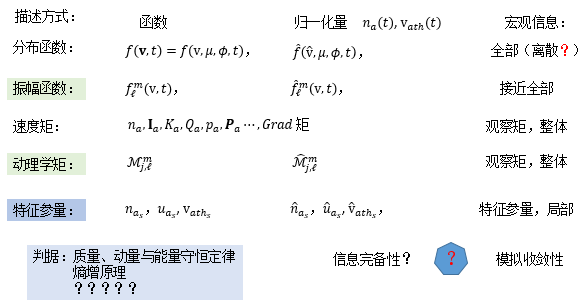
\includegraphics[width=0.8\linewidth]{figures/models/等离子体状态描述}
	\end{center}
	\caption{等离子体状态的描述:可分辨独立特征}
	\label{FigPSDisc}
  \end{figure}
  
  等离子体是由大量自由电子与带电离子为主要成分组成的统计系统。通常等离子体系统只有远小于其粒子数的独立宏观特征。例如质心系中处于热力学平衡态的等离子体系统只有两个独立特征,即密度与动理学温度。更一般地,类似于等离子体的统计系统具有如下宏观性质;记为\textbf{有限可分辨独立特征假设}。
  
  \begin{assumption} \label{假设-有限可分辨独立特征假设}
      给定可分辨独立条件\ref{假设-独立特征可分辨假设}中容差为有限大的非负小量,则有限体积、有限密度、有限温度、有限组分的等离子体系统具有有限多个可分辨独立特征。
  \end{assumption}
  
  有限多个独立特征的等离子体系统可以采用多种理论描述。然而最优理论应遵循\textbf{简单性原则},即用最少的独立参量描述同样的独立特征。根据第\ref{Fokker-Planck方程的直接解法}章的研究结果,基于有限可分辨独立特征假设\ref{假设-有限可分辨独立特征假设}并遵循理论简单性原则提出\textbf{分布函数独立特征假设}。
  
\section{分布函数独立特征假设}
\label{分布函数独立特征假设}

  \begin{theorem} \label{假说-分布函数独立特征}
      归一化分布函数满足前$l_M+1$阶振幅$\fhl \left(\rmvh \right)$收敛。根据等价原理\ref{定理-等价原理}及其推论\ref{推论-等价原理-Khlsl}可知,若第$(l,0)$阶振幅具有不大于$3N_l$个可分辨独立特征,则可用King函数为基函数$\EQ{fhlfhlsl}$表示为
      \begin{eqnarray}
          \fhl \left(\rmvh \right) &=& C_l \sum_{s=1}^{N_l} \left [ \left (\muuasl \right)^l \nhasl King \left(\rmvh;\left |\uhazsl \right |, \vhathsl \right) \right ] ~.  \label{fhlfhlslM}
      \end{eqnarray}
      当已知第$(l,0)$阶振幅函数的$3N_l$个不同$(j,l)$阶的归一化动理学矩$\calMhjlo$,则可唯一确定第$(l,0)$阶振幅函数的独立特征。其中,第$(l,0)$阶振幅的特征参量可根据任意$3N_l$个不同$(j,l)$阶的特征参量方程\EQ{MhKjl0sl}求解,
      \begin{eqnarray}
            {C_M}_j^l \sum_{s=1}^{N_l} \nhasl \vhaths^j \frac{ \uhazsl^l}{\vhathsl^l} 
            \left (1 + \sum_{k=1}^{(j-s)/2} \frac{C_{j,l}^k  \uhazsl^{2k}}{\vhathsl^{2k}} \right) = \calMhjlo , \forall l, j \ge -(l+2) ~. \label{MhKjl0slM}
      \end{eqnarray}
      常数$C_{j,l}^k$与${C_M}_j^l$分别为
      \begin{eqnarray}
          C_{j,l}^k & = & 2^k \frac{(2 l + 1)!!  C_{(j-k)/2}^k}{(2 l + 2 k + 1)!!},
          \\
          {C_M}_j^l & = & \frac{ 4 \pi}{2^{(j-l)/2}}  \frac{(l + k + 1)!!}{(2 l - 1)!!} ~.
      \end{eqnarray}
      其中,$C_{(j-k)/2}^k$是二项式系数。
  \end{theorem}
特别地,若所有阶振幅具有相同的有限个可分辨独立特征,则分布函数遵循以下\textbf{分布函数弱独立特征假设}。

  \begin{theorem} \label{假设-分布函数弱独立特征假设}
      归一化分布函数满足前$l_M+1$阶振幅$\fhl \left(\rmvh \right)$收敛。若所有阶振幅具有相同的$3N_c$个可分辨独立特征,则第$(l,0)$阶振幅可用King函数为基函数$\EQ{fhlfhls}$表示,即
      \begin{eqnarray}
          \fhl \left(\rmvh \right) &=& C_l \sum_{s=1}^{N_c}  \left [ \left (\muuas \right)^l \nhas \Kl \left(\rmvh;\left |\uhazs \right |,\vhaths \right) \right] ~.  \label{fhlfhlsM}
      \end{eqnarray}
      当已知前$l_M+1$阶振幅函数的$3N_c$个不同$(j,l)$阶的归一化动理学矩$\calMhjlo$,则可唯一确定归一化分布函数的独立特征。其中,特征参量可根据任意$3N_c$个前三阶振幅的特征参量方程\EQ{MhKjl0s}求解,
      \begin{eqnarray}
            {C_M}_j^l \sum_{s=1}^{N_c} \nhas \vhaths^j \frac{ \uhazs^l}{\vhaths^l} 
            \times  \left (1 + \sum_{k=1}^{(j-s)/2} C_{j,l}^k \frac{\uhazs^{2k}}{\vhaths^{2k}} \right) = \calMhjlo , \quad l = 0,1,2 ~. \label{MhKjl0sM}
      \end{eqnarray}
  \end{theorem}

  应用分布函数弱独立特征连续性假设\ref{假设-分布函数弱独立特征连续性假设},从定理\ref{假设-分布函数弱独立特征假设}可得到如下推论。
  \begin{corollary}\label{推论-分布函数弱独立特征}
      若服从弱独立特征假设(\ref{假设-分布函数弱独立特征假设})的归一化分布函数在随时间演化的过程中不存在特征突变,则权重系数$\nhas$可由初始条件、边界条件及推论\ref{推论-独立特征可分辨假设}共同确定;归一化分布函数具有$2N_c$个可分辨独立特征。特征参量可根据任意$2N_c$个前两阶振幅的特征参量方程\EQ{MhKjl0s}求解,
      \begin{eqnarray}
      \begin{aligned}
            {C_M}_j^0 \sum_{s=1}^{N_c} \nhas \vhaths^j 
            \times  \left (1 + \sum_{k=1}^{(j-s)/2} C_{j,0}^k \frac{\uhazs^{2k}}{\vhaths^{2k}} \right) \ = \ & \calMhj, \quad j \ge 1 . \label{MhKj00sM2}
            \\
            {C_M}_j^1 \sum_{s=1}^{N_c} \nhas \vhaths^j \frac{ \uhazs}{\vhaths} 
            \times  \left (1 + \sum_{k=1}^{(j-s)/2} C_{j,1}^k \frac{\uhazs^{2k}}{\vhaths^{2k}} \right) \ = \ & \calMhjIo , \quad j \ge -3 ~. \label{MhKj10sM2}
      \end{aligned}
      \end{eqnarray}
  \end{corollary}
  \begin{corollary}\label{推论-分布函数弱独立特征-fM}
      若服从分布函数弱独立特征假设(\ref{假设-分布函数弱独立特征假设})的归一化分布函数所有奇数阶振幅函数的归一化动理学矩都为零,即
      \begin{eqnarray}
          \calMhjlo & \equiv & 0, \quad  j \ge -(l+2), l \in 2 \bbN^+ - 1 ~.
      \end{eqnarray}
      则其独立特征的个数为$2N_c$;特征参量可根据任意$2N_c$个零阶振幅的特征参量方程\EQ{MhKjl0s}求解,
      \begin{eqnarray}
            {C_M}_j^0 \sum_{s=1}^{2N_c} \nhas \vhaths^j  = \calMhj , \quad j \ge -2 ~. \label{MhKj00sM}
      \end{eqnarray}
  \end{corollary}
  \begin{corollary}\label{推论-分布函数弱独立特征-fM-Nc}
      若服从分布函数弱独立特征假设(\ref{假设-分布函数弱独立特征假设})的归一化分布函数所有奇数阶振幅函数的归一化动理学矩皆恒为零,且权重系数$\nhas$可由初始条件、边界条件及推论\ref{推论-独立特征可分辨假设}共同确定,则归一化分布函数有$N_c$个可分辨独立特征。特征参量可根据任意$N_c$个零阶振幅的特征参量方程\EQ{MhKjl0s}求解,
      \begin{eqnarray}
            {C_M}_j^0 \sum_{s=1}^{N_c} \nhas \vhaths^j  = \calMhj , \quad j \ge 1 ~. \label{MhKj00sM1}
      \end{eqnarray}
  \end{corollary}
  
  由分布函数(弱)独立特征假设及其推论可知,当归一化分布函数具有有限个可分辨独立特征时,用归一化动理学矩描述独立特征等价于用归一化振幅函数描述这些独立特征(等价原理)。
  本章基于有限可分辨独立特征假设\ref{假设-有限可分辨独立特征假设}与分布函数弱独立特征假设\ref{假设-分布函数弱独立特征假设},针对分布函数具有弱独立特征情形,以动理学矩\EQ{MMhjlm}为变量、方程\EQ{dtfhlweak}为演化方程构造0D-2V维Fokker-Planck方程\EQ{VFPhd0D2Vaxis}的宏观矩算法。

\section{0D-2V维Fokker-Planck方程的动理学矩方程组}
\label{0D-2V维Fokker-Planck方程的动理学矩方程组}

  速度空间具有轴对称性的0D-2V维等离子体系统的归一化分布函数用Legendre多项式展开形式\EQ{FPShdlma}为
  \begin{eqnarray}
      \fh \left(\rmvh,\mu \right) &=& \sumloq \fhl \left( \rmvh \right) \Pl \left(\mu \right) ~. \label{FPShdlmaM}
  \end{eqnarray}
第$(l,0)$阶归一化振幅函数$\fhl \left( \rmvh \right)$为
   \begin{eqnarray}
       \fhl \left(\rmvh \right) & = & \int_{-1}^1 \fh \left (\rmvh, \mu \right)   \Pl (\mu) \rmd \mu, \quad l \in 0:1:l_M ~. \label{fhlLegendreM}
   \end{eqnarray}
其随时间的演化满足第$(l,0)$阶Fokker-Planck碰撞项方程\EQ{VFPhd0Dq},即
\begin{eqnarray}
    \ddt \fl &=& \ddt \left(\navth \fhl \right) \ = \ \navth \colhla (\fh, F)~.\label{VFPhd0DqM}
\end{eqnarray}
第$(l,0)$阶归一化碰撞项振幅$\colhla$是归一化分布函数$\fh\left(\rmvh,\mu \right)$与背景分布函数$F\left(\rmvhb,\mu ^{'} \right)$的非线性函数\EQ{CvlMatrix},
\begin{eqnarray}
    \left[\colhla (\rmvh) \right]_{l=0}^{l_M} &=& \colha(\rmvh,[\mub])  \cdot {\bsM}_\mu ~. \label{CvlMatrixM}
\end{eqnarray}
归一化碰撞项$\colha$的具体形式见第\ref{标量形式的非线性归一化FPS碰撞算子}节。

方程\EQ{VFPhd0DqM}关于速率的弱积分形式\EQ{dtfhlweak}为
\begin{eqnarray}
    \ddt \left[ 4 \pi m_a n_a \vath^j \int_0^\infty \rmvh^{j+2} \fhl (\rmvh) \rmd \rmvh \right] &=& 4 \pi m_a n_a \vath^j \int_0^\infty \rmvh^{j+2} \colhla (\rmvh) \rmd \rmvh 
      ~.\label{dtfhlweakM}
\end{eqnarray}
其中,
\begin{eqnarray}
    \quad -(l+2) \le j_m \le j \le j_M, \quad j \in \bbN  ~.\label{jmjM}
\end{eqnarray}
应用定义\ref{定义-归一化动理学矩}与定义\ref{定义-归一化动理学耗散力},方程\EQ{dtfhlweakM}可表述为
\begin{eqnarray}
    \ddt \left(m_a n_a \vath^j  \calMhjlo \right) &=&  m_a n_a \vath^j \calRhjlo  ~.\label{dtMhlM}
\end{eqnarray}
把方程\EQ{MMhjlm}与\EQ{RRhjlm}代入上式,化简得
\begin{eqnarray}
    \ddt \calMjlo &=& \calRjlo \ = \  m_a n_a \vath^j \calRhjlo  ~. \label{dtMl}
\end{eqnarray}
  \begin{eqnarray}
      \ddt \calMhjlo  &=& - \calMhjlo \left(\Rdtrhoa + j \Rdtvath \right) + \calRh_{j,l}^0 ~.  \label{dtMhjlM}
  \end{eqnarray}
  
  \begin{eqnarray}
      \ddt \calMhj  &=& -  \calMhj \left(\Rdtrhoa + j \Rdtvath \right) + \calRh_{j,0}^0 ~.  \label{dtMhj0M}
  \end{eqnarray}
此即由于受到Coulomb碰撞作用,组分$a$的第$(j,l,0)$阶动理学矩随时间演化方程。


\subsection{Coulomb碰撞过程}
\label{Coulomb碰撞过程}

本文采用非线性FPS碰撞算子\EQ{FPShdabSi}。记方程\EQ{dtfhlweakM}中第$k$时间步的碰撞项振幅$\colhla (\rmvh,t_k)$的计算过程为第$k$个碰撞步,具体如下。首先,根据第$k$步的动理学矩$\calMjlo(t_k)$求出第$k$步分布函数的归一化振幅函数$\fhl \left(\rmvh,\tk \right)$。

第$k$时间步的第$(j,l,0)$阶归一化动理学矩为
  \begin{eqnarray}
      \calMhjlo (\tk) &=& \rho_a^{-1} \vath^{-j} \calMjlo (\tk) ~. \label{Mhjlk}
  \end{eqnarray}
基于有限可分辨独立特征假设\ref{假设-有限可分辨独立特征假设},根据分布函数弱独立特征假设\ref{假设-分布函数弱独立特征假设}及其推论\ref{推论-分布函数弱独立特征},组分$a$的分布函数具有$2N_c$个可分辨独立特征;特征参量满足方程\EQ{nuThsMhjl},即
      \begin{eqnarray}
      \begin{aligned}
            {C_M}_j^0 \sum_{s=1}^{N_c} \nhas \vhaths^j 
            \times  \left (1 + \sum_{k=1}^{(j-s)/2} C_{j,0}^k \frac{\uhazs^{2k}}{\vhaths^{2k}} \right) \ = \ & \calMhj\left(\tk \right), \quad j \ge 1 . \label{MhKj00sM2k}
            \\
            {C_M}_j^1 \sum_{s=1}^{N_c} \nhas \vhaths^j \frac{ \uhazs}{\vhaths} 
            \times  \left (1 + \sum_{k=1}^{(j-s)/2} C_{j,1}^k \frac{\uhazs^{2k}}{\vhaths^{2k}} \right) \ = \ & \calMhjIo\left(\tk \right) , \quad j \ge -3 ~. \label{MhKj10sM2k}
      \end{aligned}
      \label{MhKjl0sM2k}
      \end{eqnarray}
特征参量方程中阶数集$[j]$的选取不唯一。本文采用如下奇奇偶偶格式,
\begin{align*}
\begin{split}
    j = \left \{
    \begin{array}{lr}
          2:2:2N_c,      & l=0 \\
          1:2:2N_c-1,    & l=1
    \end{array} ~.
\right.
\end{split}
\end{align*}
此时,特征参量方程\EQ{MhKjl0sM2k}为$2N_c$个非线性代数方程构成的适定方程组。采用\textbf{最小二乘法}(LSM,Least Square Method)解方程\EQ{MhKjl0sM2k},可唯一确定一组归一化振幅函数\EQ{fl0sk}的特征参量,即$2N_c$个$\uhazs$与$\vhaths$。分布函数的第$(l,0)$阶归一化振幅$\fhl \left(\rmvh,t \right)$可用King函数\EQ{fhlfhlsM}表示。

采用步长为$\Dvha=\rmvh_{a_M} / 2^{n_2}, n_2 \in N^+$建立以$[\rmvhA], \alpha = 1:2^{n_2}+1$为节点的均匀背景网格,则在节点$\rmvhA$上第$(l,0)$阶归一化振幅为
\begin{eqnarray}
    \fhl \left(\rmvhA,\tk \right) &=& C_l \sum_{s=1}^{N_c} \left [ \left (\muuas \right)^l \nhas \Kl \left(\rmvhA;\left |\uhazs \right | , \vhaths \right) \right ]  ~.  \label{fl0sk}
\end{eqnarray}
其中,权重系数$\nhas$根据初始条件、边界条件及推论\ref{推论-独立特征可分辨假设}共同确定。基于方程\EQ{fl0sk}采用自动微积分计算归一化分布函数对速度轴的偏导数、采用映射\EQ{FLMmapping}计算背景分布函数在节点$[\rmvh_{b_\alpha}]$上的插值函数$\FhL \left([\vvbth_\alpha] \right)$。则第$k$时间步在节点$\rmvhA$上有
  \begin{eqnarray}
  \begin{aligned}
      \ddrmvh \fhl \left(\rmvhA, \tk \right) \quad \approx \quad & \ddrmvh \scrfhl \left(\rmvhA, \tk \right),
      \\
      \dddrmvh \fhl \left(\rmvhA, \tk \right) \quad \approx \quad & \dddrmvh \scrfhl \left(\rmvhA, \tk \right) ,
      \\
      F_L^0 mapping:\FhL \left(\rmvh_{b_\alpha}, \tk \right) \to \quad & \FhL \left(\vvbth_\alpha, \tk \right) ~. \label{FL0mappingAM}  
  \end{aligned}
  \end{eqnarray}
  
  基于$\FhL \left([\vvbth_\alpha], \tk \right)$,采用第\ref{Rosenbluth势的数值积分法}节的过程计算Rosenbluth势函数的振幅及其关于$\vvbth$的前两阶偏导数;并与方程\EQ{fl0sk}-\EQ{FL0mappingAM}一起代入第\ref{标量形式的非线性归一化FPS碰撞算子}节给出第$k$步的归一化碰撞项$\colha\left(\rmvhA, \tk \right)$。
  第$(l,0)$阶归一化碰撞项振幅满足方程\EQ{CvlMatrix},在第$\alpha$个节点上有
   \begin{eqnarray}
        \left[\colhla (\rmvhA, \tk) \right]_{l=0}^{l_M} &=& \colha(\rmvhA,[\mub], \tk)  \cdot {\bsM}_\mu ~. \label{CvlMatrixAM}
   \end{eqnarray}
  % 应用关系\EQ{colhacola},则第$k$时间步在节点$\rmvhA$上的第$(l,0)$阶碰撞项振幅为
  % \begin{eqnarray}
  %     \colla \left(\rmvhA,\tk \right) &=& \frac{n_a}{\vath^3}  \colhla \left(\rmvhA,\tk \right) ~.\label{colacolhak}
  % \end{eqnarray}
  % 把上述方程代入方程\EQ{Rjlm}并
  采用Romberg积分法(文献)计算积分\EQ{Rhjlm}并代入方程\EQ{dtMl},则第$k$步的第$(l,0)$阶动理学矩随时间的变化率为
  \begin{eqnarray}
      \ddt \calMjlo \left(\tk \right) &=& \calRjlo \left(\tk \right)  \ = \  m_a \nak \vathk^j \calRhjlo \left(\tk \right) ~.\label{ddtMjl0}
  \end{eqnarray}
  \begin{eqnarray}
      \ddt \calMhjlo  &=& - \calMhjlo \left(\Rdtrhoa + j \Rdtvath \right) + \calRh_{j,l}^0 ~.  \label{ddtMhjl0}
  \end{eqnarray}

\subsection{时间积分}
\label{宏观矩法时间积分}

方程\EQ{dtMl}两边在区间$[\tk,\tkI]$上对时间积分,有
  \begin{eqnarray}
      \calMjlo \left(\tkI \right) & = & \calMjlo \left(\tk \right) +  \int_{\tk}^{\tkI} \calRjlo \left(\tau \right) \rmd \tau ~. \label{MjloRk1}
  \end{eqnarray}
  
  \begin{eqnarray}
      \calMhjlo \left(\tkI \right)  &=& \calMhjlo \left(\tk \right) - j   \int_{\tk}^{\tkI} \calMhjlo \Rdtvath \rmd \tau +    \int_{\tk}^{\tkI} \calRhjlo \rmd \tau ~.
  \end{eqnarray}
  \begin{eqnarray}
      \calMhjlo \left(\tkI \right)  &=& \calMhjlo \left(\tk \right) - j   \int_{\tk}^{\tkI} \calMhjlo \left(\tau \right) \ddtau \ln{\vath} \rmd \tau +    \int_{\tk}^{\tkI} \calRhjlo \left(\tau \right) \rmd \tau ~.  \label{MhjloRhk1}
  \end{eqnarray}
  \begin{eqnarray}
  \begin{aligned}
      \left(1 + j  \ln{\vathkI} \right) \calMhjlo  \ =& \ \left(1 + j  \ln{\vathk} \right) \calMhjlo \left(\tk \right)  
      \\
      + & j   \int_{\tk}^{\tkI} \ln{\vath} \ddtau \calMhjlo \left(\tau \right)  \rmd \tau 
      \\
      + &   \int_{\tk}^{\tkI} \calRhjlo \left(\tau \right) \rmd \tau ~.
  \end{aligned}
  \end{eqnarray}
  \begin{eqnarray}
  \begin{aligned}
       \calMhjlo  \ =& \  \frac{1 + j \ln{\vathk}}{1 + j \ln{\vathkI}} \calMhjlo \left(\tk \right)  
      \\
      - & \frac{j^2}{2\left(1 + j \ln{\vathkI} \right)}   \int_{\tk}^{\tkI} \calMhjlo \ddtau \left(\ln{\vath} \right)^2  \rmd \tau  
      \\
      + & \frac{1}{1 + j \ln{\vathkI}} \int_{\tk}^{\tkI} \left(1 + j \ln{\vath} \right) \calRhjlo \rmd \tau ~.
  \end{aligned}
  \end{eqnarray}
  
\begin{definition} \label{定义-动理学广义冲量}
    第$(j,l,0)$阶\textbf{动理学耗散冲量}是第$(j,l,0)$阶动理学耗散力的时间泛函,有
    \begin{equation}
        \calIjlo \left(t;t_0 \right) \ = \ \int_{t_0}^t \calRjlo \left(\tau \right) \rmd \tau ~. \label{IRjl}
    \end{equation}
   \end{definition}
\noindent
此即由于受到背景粒子Coulomb散射,从$t_0$到$t$时刻组分$a$在$z$方向引起的第$(j,l,0)$阶冲量变化量。特别地,当$j=l=1$时,上式为
      \begin{equation}
        \calI_{1,1}^0 \left(t;t_0 \right) \ = \ \int_{t_0}^t \calR_{1,1}^0 \left(\tau \right) \rmd \tau ~. \label{IR110}
      \end{equation}

应用定义\ref{定义-动理学广义冲量},则第$k+1$时间步的第$(j,l,0)$阶归一化动理学矩可表述为
  \begin{eqnarray}
      \calMjlo \left(\tkI \right) & = & \calMjlo \left(\tk \right) +  \Dtk  \calIjlo \left(\tkI; \tk \right) ~. \label{Mjlmk1}
  \end{eqnarray}
  动理学耗散冲量\EQ{IRjl}是以碰撞项为被积函数、时间$t$与速度$\v(\rmv,\mu,\phi)$为变量的四维积分。
  
  方程\EQ{Mjlmk1}中第$(l,m,0)$阶动理学耗散冲量$\calIjlo \left(\tkI; \tk \right)$可采用标准\textbf{Runge-Kutta}方法计算。采用一阶显式格式(\textbf{显式Euler})时,第$(l,m,0)$阶动理学耗散冲量$\calIjlo \left(\tkI; \tk \right)$为
  \begin{eqnarray}
      \calIjlo \left(\tkI; \tk \right) &\approx& \Dtk \calRjlo \left(\tk \right) ~. \label{Ijlokk1RK1exM}
  \end{eqnarray}
  其中,$\Dtk=\tkI-\tk$。
  采用\textbf{隐式Euler}方法时,有
  \begin{eqnarray}
      \calIjlo \left(\tkI; \tk \right) &\approx& \Dtk \calRjlo \left(\tkI \right) ~. \label{Ijlokk1RK1imM}
  \end{eqnarray}
  采用\textbf{二阶显式Heun}格式时有
  \begin{eqnarray}
      \calIjlo \left(\tkI; \tk \right) &\approx& \frac{\Dtk}{2} \left[\calRjlo \left(\tk \right) + \calRjlo \left(\tkI \right)\right] ~. \label{Ijlokk1RK2exM}
  \end{eqnarray}
  隐式Euler与显式Heun格式需用显式Euler法做第一步计算,给出$k+1$步预估的动理学耗散力。基于二阶显式Heun格式可构造$N_2$次$\calRjlo(\tkI)$迭代的二阶隐式Runge-Kutta方法,即\textbf{梯形法}。

  第$k+1$时间步的动理学热速度有两种方法计算。其一是采用如下离散格式
  \begin{eqnarray}
      \RvathkI &=& \frac{\vathkI}{\vathk} \ = \ \sqrt{1 - \frac{2}{3} \Dtk \left [\Dtk \left(\delta_t \Izak \right)^2 - \scrW_k \right ]  }. \label{Rvathk1}
  \end{eqnarray}
  式中,函数$\scrW$与速度空间坐标无关的宏观量,
  \begin{eqnarray}
      \scrW &=&  \calRh_{2,0}^0 - \frac{2}{3} \uzha \calRh_{1,1}^0 .   \label{scrW}
  \end{eqnarray}
  组分$a$的第$k$时间步相对动量变化率以及相对总能量变化率分别为
  \begin{eqnarray}
      \delta_t \Izak &=& \frac{1}{m_a \nak \vathk} \ddt \Izak \ = \  \ddt \uzhak + \uzhak \Rdtvathk , \label{RdIak}
      \\
      \delta_t \Kak &=& \frac{1}{\nak \Tak} \ddt \Kak \ = \ 2 \uzhak \ddt \uzhak + \left(3 + 2  \uzhIIak \right) \Rdtvathk ~. \label{RdKak}
  \end{eqnarray}
其中,
  \begin{eqnarray}
      \ddt \uzhak  &=&  \frac{1}{3} {\calRh_{1,1}^0}{_k} ~. \label{ddtuzhak}
  \end{eqnarray}
  当碰撞步具有收敛的数值结果,即满足
  \begin{eqnarray}
      \left|\ddt \nak \right| + \left|\ddt \nbk \right| &=& 0 , \label{dnabk}
      \\
      \ddt \Izak + \ddt \Izbk &=& 0 , \label{dIabk}
      \\
      \ddt \Kak + \ddt \Kbk &=& 0 ~, \label{dKabk}
  \end{eqnarray}
  则格式\EQ{Rvathk1}满足约束方程\EQ{vathKu}以及离散守恒,则本文的宏观矩算法具有离散的质量守恒、动量守恒与能量守恒。

  第二种方法是直接根据约束方程\EQ{vathKu}计算$k+1$时间步的动理学热速度,即
      \begin{eqnarray}
        \vath \left(\tkI \right) &=& \sqrt{\frac{2}{3} \left (\frac{2 \KakI}{m_a \nakI \uzakI} - \uzakI^2 \right)} ~. \label{vathKuk}
      \end{eqnarray}
  隐式迭代算法的整体收敛性可采用如下判据
  \begin{eqnarray}
      \left|\frac{\vath \left(\tkI \right)}{\vathkI}  - 1 \right| \le rtol ~.
  \end{eqnarray}
  通过数值收敛性分析可知,格式\EQ{Rvathk1}是格式\EQ{vathKuk}的一阶近似。本文采用第二种格式\EQ{vathKuk}计算动理学热速度。
  
\section{数值算例}
\label{宏观矩法数值算例}

  
\chapter{Fokker-Planck方程的特征参量法}
\label{Fokker-Planck方程的特征参量法}

\section{叠加原理}

\begin{eqnarray}
    \ddt {\calMjlo}_s &=& \sum_{s=1}^{2(N_{c_a}+N_{c_b})} {\calRjlo}_s ~.\label{dtMl-sum}
\end{eqnarray}

  \begin{corollary}\label{推论-分布函数弱独立特征演化矩阵}
      根据推论(\ref{推论-分布函数弱独立特征})可得特征参量随时间的演化方程:
      \begin{eqnarray}
            \bsA \cdot \ddt \bfx & = & \bfb . \label{Axb-dtuTs}
      \end{eqnarray}
      其中,
      \begin{eqnarray}
            \bfx & = & \left[\uazI, \vathI, \cdots, \uazs, \vaths, \cdots \right]^T , \label{bfx-uTs}
            \\ 
            \bfb & = & \left[\ddt {\calM}{_{1,1}^0}, \ddt {\calM}{_{2,0}^0}, \ddt {\calM}{_{3,1}^0}, \ddt {\calM}{_{4,0}^0}, \cdots, \ddt {\calM}{_{2N_c+1,1}^0}, \ddt {\calM}{_{2N_c+2,0}^0} \right]^T , \label{bfb-dtMj00}
      \end{eqnarray}
      矩阵$\bsA$是根据特征参量方程\EQ{MhKj10sM2}求$\partial_t \bfx$时对应的质量矩阵。
  \end{corollary}
  
      \begin{eqnarray}
            \ddt \bfx & = & \bsA^{-1} \cdot \bfb . \label{xAb-dtuTs}
      \end{eqnarray}
  1
  % 在Lagrange坐标系中,
\begin{theorem} \label{假设-独立特征可分辨假设-dtIK}
    若基函数$ \Kl \left(\rmv;{\mu}_1 ,{\sigma}_1 \right) $与$ \Kl \left(\rmv;{\mu}_1 ,{\sigma}_1 \right) $ 满足互碰撞模型\EQ{VFPhd0DqM}的相对动量变化率 ${\partial}_t I $ 与相对能量变化率 ${\partial}_t K $ 是一个可忽略的小量,即
    \begin{eqnarray}
      \frac{1}{K} \left| \ddt K \right| & \le & rtol , \label{RdtKs}
      \\ 
      \frac{1}{\left| I \right| + eps} \left| \ddt I \right|  & \le & rtol, \label{RdtIs}
    \end{eqnarray}
    则两组特征参量$\left(\mu_1,\sigma_1 \right)$与$\left(\mu_2,\sigma_2 \right)$不可分辨;否则,称其为\textbf{可分辨独立特征}。
\end{theorem}
\noindent
方程\EQ{RdtKs}与\EQ{RdtIs}是独立特征不可分辨条件的变化率形式,记为第二类独立特征可分辨判据。
定理\ref{假设-独立特征可分辨假设-dtIK}等价于定理\ref{假设-独立特征可分辨假设},是以特征参量变化率表述的独立特征可分辨假设。

\section{0D-2V维Fokker-Planck方程的特征参量方程组}
\label{0D-2V维Fokker-Planck方程的特征参量方程组}

\section{时间积分}
\label{特征参量时间积分}

\section{数值算例}
\label{特征参量法数值算例}


\chapter{Coulomb对数}
\label{Coulomb对数}

\chapter{Fokker-Planck方程的神经网络增强特征参量法}
\label{Fokker-Planck方程的神经网络增强特征参量法}

\section{特征参量的基因网络}
\label{特征参量的基因网络}

\section{0D-2V维Fokker-Planck方程的神经网络增强特征参量法}
\label{0D-2V维Fokker-Planck方程的神经网络增强特征参量法}

\section{时间积分}
\label{神经网络增强特征参量法时间积分}

\section{数值算例}
\label{神经网络增强特征参量法数值算例}





\chapter{快粒子在均匀背景等离子体中慢化}
\label{快粒子在均匀背景等离子体中慢化}

快粒子在等离子体的演化是磁约束聚变燃烧等离子体中的重要物理问题。首先,中性束注入、电子回旋波加热或者离子回旋波加热是托卡马克、场反箍缩等磁约束聚变方案实现点火的重要加热技术。由于直接注入加热或者共振加热等,以电子、氘与氚等组成的背景等离子体中产生高能尾巴。这些高能尾巴中的快粒子由于受到Coulomb散射以及等离子体中平均场效应的影响,在等离子体中不断慢化与热化并把部分动量与能量传递给背景等离子体。另外,在燃烧等离子体中,氘与氚 (或者质子与硼离子) 聚变反应过程中产生能量高达几个 MeV 的α粒子。对这些快粒子在等离子体中的慢化与热化过程的研究有助于对加热过程及燃烧物理的理解。

\section{聚变α 粒子在背景均匀等离子体中慢化}

\section{粒子束在背景均匀等离子体中慢化}

% !TeX root = ../main.tex










\chapter{Vlasov-Fokker-Planck方程的分裂算法}

  由于碰撞项方程不满秩所谓哈密顿方程,使得 VFP 方程在一般情形为非保守哈密顿系统。然而当忽略虑碰撞项时,VFP 方程约化为 Vlasov 方程。Vlasov 方程与描述电磁场演化的 Maxwell 方程组成Maxwell-Vlasov系统。Maxwell-Vlasov 系统是一种 Hamilton 系统;Hamiltonian 分裂法是数值求解的一种有效算法。
  
\section{Hamiltonian 分裂法}

  定义函数 $\mathscr{F}$ 与 $\mathscr{G}$ 在无限维流形空间 $\mathscr{M}=\left\{\left(f,\bfE,\bfB \right)| \ddbfv \cdot \bfB = 0 \right\} $,则 Morrision-Marsden-Weinstein(MMW)括号定义为
  \begin{equation}
  \begin{aligned}
      \left\{\mathscr{F},\mathscr{G} \right \} \ = \ & {\int \int}_{\Omega} f \left[\frac{\delta \mathscr{F}}{\delta f},\frac{\delta \mathscr{G}}{\delta f} \right]_{\bfx \bfv} \rmd \bfx \rmd \bfv + 
      {\int \int}_{\Omega} f \bfB \left(\ddbfv \frac{\delta \mathscr{F}}{\delta f} \times \ddbfv \frac{\delta \mathscr{G}}{\delta f} \right) 
      \\
      + & {\int \int}_{\Omega} \left(\frac{\delta \mathscr{F}}{\delta \bfE} \cdot \ddbfv f \frac{\delta \mathscr{G}}{\delta f} -
      \frac{\delta \mathscr{G}}{\delta \bfE} \cdot \ddbfv f \frac{\delta \mathscr{G}}{\delta f}\right) \rmd \bfx \rmd \bfv 
      \\
      + & \int_{\Omega} \left[\frac{\delta \mathscr{F}}{\delta \bfE}  \cdot \left(\nabla \times \frac{\delta \mathscr{G}}{\delta \bfB} \right) - \frac{\delta \mathscr{G}}{\delta \bfE}  \cdot \left(\nabla \times \frac{\delta \mathscr{F}}{\delta \bfB} \right) \right ] ~.
  \end{aligned}
  \end{equation}
  其中,$\left[\cdot,\cdot \right]_{\bfx \bfv}$ 代表以 $\left(\bfx,\bfv \right)$ 为宗量的两个函数的正则Lie括号,形如
  \begin{eqnarray}
      \left[h \left(\bfx,\bfv \right),g \left(\bfx,\bfv \right)  \right]_{\bfx,\bfv} &=& \sum_{i=1}^3
      \left(\frac{\partial h}{\partial x_i} \frac{\partial g}{\partial \rmv_i} - \frac{\partial g}{\partial x_i} \frac{\partial h}{\partial \rmv_i}  \right) ~.
  \end{eqnarray}
  文献证明了方程()是Poisson括号。定义 $\mathscr{M}$ 流形空间中 $\mathscr{Z}=\left(f,\bfE,\bfB \right)$,此时Vlasov-Maxwell可用上述定义表示为
  \begin{eqnarray}
      \ddt \ = \ \left\{\mathscr{Z},\mathscr{H} \right \} ~.
  \end{eqnarray}
  其中,Vlasov-Maxwell 系统的 Hamiltonian 函数为
  \begin{eqnarray}
      \mathscr{H} \left(f,\bfE,\bfB  \right) \ = \ \frac{1}{2} \epsilon_r \int_{\Omega} \left |\bfE \right|^2 \rmd \bfx + \frac{1}{2 \mu_0}  \int_{\Omega} \left |\bfB \right|^2 \rmd \bfx + \frac{m_a}{2} \epsilon_r \int \int_{\Omega} \left |\v \right|^2 f \rmd \bfx \rmd \bfv~.
  \end{eqnarray}
  


\section{1D-2V维多组分VFP方程的无网格算法}
\label{1D-2V维多组分VFP方程的无网格算法}

  

\section{数值算例}


\chapter{结束语}

\section{主要观点与工作}

伪谱法作为谱分析方法,求解光滑函数时具有指数收敛性,该性质使得可以用较少的格点获得较高的数值精度。利用系统的内在对称性通常可以简化理论的复杂性。等离子体由于受到Coulomb碰撞作用,分布函数在速度空间通常具有较好的光滑性;Coulomb碰撞过程在速度空间具有球对称性。另外,归一化通常可提高算法的数值稳定性。因此在速度空间中,选择球谐函数作为基函数,用伪谱法相关系数计算导数,求解归一化的Rosenbluth-Fokker-Planck方程,可以获得较高的计算效率与准确性。

伪谱法另一个大优点是应用于非线性问题时易于构造以及编程实现,因此被广泛研究并应用到解光滑的非线性问题。然而经典伪谱法也有两个不足:第一,当有网格映射时,若映射前后网格差异性很大(本质是光滑性不足),经典伪谱法求解效率与准确性都显著降低;第二,伪谱法只能快速收敛到理论值附近,因此通常难以直接构造守恒格式。

本文通过在速度轴方向使用自适应网格技术,提出了一种角度方向使用经典伪谱法、速度轴方向在自适应优化的网格上应用有限差分法的混合算法;并基于后验分析方法,构造满足离散守恒的自适应增强伪谱法。本算法相较于传统算法有一定比较优势:
1.	改善了传统伪谱法对于光滑性过于敏感的缺点;
2.	可以优化出比分步所用局域法(本文是二阶有限差分)具有高一阶甚至两阶的收敛速率,称之为“超收敛”。
3.	满足了离散守恒性,并且可以方便地推广到更高阶矩;
综合计算效率、准确性、适用性以及鲁棒性等性能指标,本算法是一个综合得优的方案。

当物理空间结合有限体积法,可以推广大六维相空间解VFP方程。由于实现了离散守恒并保留了速度空间所有非线性项,因此本算法适合于模拟燃烧等离子体产生的高能α粒子慢化、加热驱动的高能尾巴的耗散等多尺度非线性问题。


\section{总结与展望}

随着稳态燃烧等离子体的演化逐渐成为要面对的科学问题,先前惯用的小尺度、线性化研究方法会渐渐倍感吃力。大尺度、非线性等离子体演化通常同时存在不同的运动模式;由于电磁作用力是长程力的属性,这些模式通常会有不同程度的耦合。解决这类复杂多尺度物理问题,通常近似方法难以给出更全面的物理图像。而且这类系统的演化多具有大时间尺度、大计算量的特点,因而算法的计算效率、长时间的稳定性以及满足离散守恒性成为等离子体模拟算法的关键指标。传统局域方法(如有限差分等)以及经典谱方法已无法满足等离子体模拟中日益增长的需求,基于后验分析构造的满足离散守恒要求的自适应伪谱算法正是为解决这一挑战而提出。本文的核心思想是把局域方法与伪谱法深度融合构造综合更优的算法,且各个子步骤可以独立优化。目前所构造的离散守恒的自适应伪谱算法求解Rosenbluth-Fokker-Planck方程时,经过了多组分(e-D-T-α)、多参量(质量、密度、温度、平均速度等)、大参数区间(4个数量级)、长时间尺度(上百个碰撞特征时间)的验证。结合物理空间有限体积法进一步推广到VFP方程,有潜力对燃烧等离子体、强流束与等离子体相互作用、磁重联等问题进行研究。

本文的主要贡献是:验证了完全非线性的用球谐函数展开的碰撞项方程可以求解,采用自适应网格技术以及后验分析方法,构造了多步、显式、满足离散守恒的非线性收敛的伪谱算法,验证了算法具有超收敛性。

更重要的,本文提出的算法本质是一种优化策略。自然,目前还有很多不足之处:

	速度空间中,现在采用的自适应网格优化伪谱法,本质上速度轴方向是二阶有限差分法(现在可达到2~4阶的超收敛)。目前只是简单应用倍增自适应细化方案,自适应性还太弱,可以采用更高效的自适应方案。
 
	伪谱法本身可以继续优化。在控制领域有各种优化的伪谱法,如Bellmann伪谱法。其基本思想是,把初始Gaussian配置点根据系统特点做某种变换,然后基于变换后的non-Gaussian配置点应用Bellmann伪谱法。若此方法可行,则不需要上面自适应网格优化并引入有限差分法了。整个速度空间用以完全采用伪谱法,将有接近指数收敛性。
 
本质上,上面两种方案都是优化;只是第一种具有更好的适应性;第二种具有更快的收敛性。中间也许存在综合最优方案。

	后验分析方法构造离散守恒时,我们目前只是用最简单的二分机制吸收残差。更严谨的理论是流形映射,也已经是一个蓬勃发展的领域了,有各种更映射方案。另外此方案可方便地推广到高阶矩守恒,这个对湍流等需要高阶矩的研究可能有帮助。
 
	物理空间中,现在有限体积法使用的是结构化网格。多重网格技术来可作为对立算法,也可作为预求解器加速其他算法。 这对于将来做五维研究(甚至解六维VFP方程)会很重要。
 
这几方面是比较明确且有良好预期的优化方向,进一步构造具有高的计算效率、强的适用性、低的累积误差、高的准确性的守恒算法是一个充满挑战而值得研究的问题。这一块也是今后工作的一个重点。

